\documentclass[10pt]{beamer}
\usepackage[utf8]{inputenc}

\usepackage{multirow,rotating}
\usepackage{color}
\usepackage{tikz-cd}
\usepackage{array}
\usepackage{siunitx}
\usepackage{mathtools,nccmath}%
\usepackage{etoolbox, xparse} 
\usepackage{amsfonts}
\usepackage{amssymb}
\usepackage{amsthm}
\usepackage{amsmath}
\usepackage{amsopn}
\usepackage{pifont}
\usepackage{xcolor}
\usepackage{booktabs}
\usepackage{float}
\usepackage{epstopdf}
\usepackage{tikz}
\usepackage{graphicx}
\usepackage{subcaption}
\usepackage{hyperref}

\usetikzlibrary{positioning,backgrounds, arrows.meta}

\epstopdfDeclareGraphicsRule{.tif}{png}{.png}{convert #1 \OutputFile}
\AppendGraphicsExtensions{.tif}

\usetheme{CambridgeUS}
\usecolortheme{dolphin}
\makeatletter

\setbeamertemplate{footline}{%
    \hfill{\fontsize{8pt}{16pt}\selectfont\insertframenumber}\hspace{2em}\vspace{1em}
}


\newenvironment{hidepagenumberframe}
  {\setbeamertemplate{footline}{}\begin{frame}}
  {\end{frame}\setbeamertemplate{footline}{
     \hfill{\fontsize{8pt}{16pt}\selectfont\insertframenumber}\hspace{1em}}}


\makeatother


\setbeamertemplate{caption}[numbered]

% set colors
\definecolor{myNewColorA}{RGB}{158, 27,50}
\definecolor{myNewColorB}{RGB}{158, 27,50}
\definecolor{myNewColorC}{RGB}{158, 27,50} % {130,138,143}
\setbeamercolor*{palette primary}{bg=myNewColorC}
\setbeamercolor*{palette secondary}{bg=myNewColorB, fg = white}
\setbeamercolor*{palette tertiary}{bg=myNewColorA, fg = white}
\setbeamercolor*{titlelike}{fg=myNewColorA}
\setbeamercolor*{title}{bg=myNewColorA, fg = white}
\setbeamercolor*{item}{fg=myNewColorA}
\setbeamercolor*{caption name}{fg=myNewColorA}
\setbeamercolor*{button}{bg=myNewColorA,fg= white}
\definecolor{rougeprez}{RGB}{158,27,50}
% Remove the button from appearing
%\setbeamertemplate{button}{}

% Disable navigation symbols
\setbeamertemplate{navigation symbols}{}

% Disable button template
%\setbeamertemplate{button}{}

% Optional: Remove footline (if needed)
%\setbeamertemplate{footline}{}

\setbeamercolor{date in head/foot}{fg=white}


\usefonttheme{professionalfonts}

\definecolor{babyblueeyes}{rgb}{0.63, 0.79, 0.95}
\definecolor{apricot}{rgb}{0.98, 0.81, 0.69}
\definecolor{grannysmithapple}{rgb}{0.66, 0.89, 0.63}
\definecolor{carnationpink}{rgb}{1.0, 0.65, 0.79}
\definecolor{brilliantlavender}{rgb}{0.96, 0.73, 1.0}

\usepackage{natbib}

%------------------------------------------------------------
% \titlegraphic{\includegraphics[height=0.75cm]{ua_eng_logo.png}} 

% logo of my university


%\titlegraphic{%
%\includegraphics[width=3.0cm]{ua_seal.png}
%}

\setbeamerfont{title}{size=\large}
\setbeamerfont{subtitle}{size=\small}
%\setbeamerfont{author}{size=\small}
\setbeamerfont{date}{size=\footnotesize}
\setbeamerfont{institute}{size=\footnotesize}

%\date[\textcolor{white}{Conference Name, 2022}]
%{Conference full name\\
%Aug 29-30, 2022}

%------------------------------------------------------------
%This block of commands puts the table of contents at the 
%beginning of each section and highlights the current section:
%\AtBeginSection[]
%{
%  \begin{frame}
%    \frametitle{Contents}
%    \tableofcontents[currentsection]
%  \end{frame}
%}
%\AtBeginSection[]{
 % \begin{frame}
 % \vfill
  %\centering
  %\begin{beamercolorbox}[sep=8pt,center,shadow=true,rounded=true]{title}
    %\usebeamerfont{title}\insertsectionhead\par%
 % \end{beamercolorbox}
  %\vfill
  %\end{frame}

% ------Contents below---
%------------------------------------------------------------

\begin{document}
\author[I. Barriola, R. Chaba]{I. Barriola\inst{1} \and R. Chaba\inst{2}}

\institute{
	\inst{1} CRED, Paris Panthéon Assas University, Paris, France
	\and
	\inst{2} LEMMA, Paris Panthéon Assas University, Paris, France
}
\title{The Death of Distance: Mobile Internet and Political Trust in Africa}
\subtitle{Working Paper}
\date{February 3, 2025}


\begin{hidepagenumberframe}
    \titlepage
\end{hidepagenumberframe}

\begin{frame}{Context}
    \begin{quotation}
        \noindent \textbf{``The State stops at PK 12, twelve kilometers from the capital, Bangui.''}\\       
        \hfill -- A Central African Republic official \textcolor{gray}{\textit{(Bierschenk \& Olivier de Sardan, 1997)}} 
        \end{quotation}\smallskip \pause

    \begin{itemize}\setlength\itemsep{1em}
        \item Broader pattern of spatial disparity in state presence across Africa: state presence diminishes sharply with distance from
        capital cities \vfill \pause
        \item Colonial powers’ strategic placement of capital cities in \hyperlink{sample_map}{{peripheral locations}}
        \vfill \label{context}
        \begin{itemize}
            \item Most former colonial capitals became modern national capitals \vfill
            \item Persistent disparities in how African states
            interact with their populations \textcolor{gray}{\textit{Lewis, 1954; Bates, 1983}} \vfill
            \item Centralization formalized in 80\% of African constitutions \textcolor{gray}{\textit{Kuperman, 2015}} \vfill  \pause
        \end{itemize} 
        \item As distance from the capital
        increases, national institutions struggle to project their authority, leading to systematic
        variations in state presence \textcolor{gray}{\textit{Migdal, 1988; Herbst, 2000; Michalopoulos and Papaioannou,
        2014}} \vfill   \pause
        \vspace{1em}
        \centering Shape how citizens develop trust in political institutions, depending on their proximity to the capital city \vfill
    \end{itemize}
\end{frame}


\begin{frame}{Motivation}
        \centering Spatial variation in state presence creates two interrelated challenges that shape citizens’ relationship
        with political institutions\vfill   \pause
        \smallskip
        \setbeamertemplate{enumerate items}[default]

        \begin{enumerate}
            \item Information scarcity in remote areas alters how citizens process and respond to political information\vfil
            \begin{itemize}\setlength\itemsep{1em}
                \vspace{0.5em}
                \item Given the high costs of acquiring reliable information about government performance, citizens rationally adapt by relying
                on accessible but potentially biased sources: ethnic affiliations, partisan signals, and local
                social networks \textcolor{gray}{\textit{McKay et al., 2023; Brinkerhoff et al., 2018}}\vfill   \pause
                \item Without exposure to comparative benchmarks, these citizens lack reference points
                for evaluating public service quality, often normalizing suboptimal outcomes as the status
                quo \textcolor{gray}{\textit{Adida et al., 2020; Gottlieb, 2016; Provenzano, 2024}}\vfill
               \end{itemize}
            \end{enumerate}
        \end{frame}

\begin{frame}{Motivation}
    \setbeamertemplate{enumerate items}[default]

    \begin{enumerate}
        \setcounter{enumi}{1}
        \item Self-reinforcing cycle of low expectations and reduced engagement
        \begin{itemize}\setlength\itemsep{1em}
            \vspace{0.5em}
            \item Infrequent interactions with state institutions and officials lead citizens to downgrade their expectations
            of government capacity and responsiveness \textcolor{gray}{\textit{McKay et al., 2023; Brinkerhoff et al., 2018}}   \pause
            \item Systematic detachment from the state institutions develop
            a form of rational inattention: citizens who rarely encounter state services have little
            incentive to invest in monitoring government performance   \pause
            \item Physical and psychological
            distance from the capital further weakens national identification, creating a disconnect between
            remote populations and central institutions \textcolor{gray}{\textit{Michalopoulos and Papaioannou, 2014;
            Campante et al., 2019; Brinkerhoff et al., 2018; McKay et al., 2023}}\vfill   \pause
        \end{itemize}
    \end{enumerate}

    \centering These dynamics converge into an equilibrium of uninformed, disengaged trust in remote areas that undermines political accountability \vfill
\end{frame}




\begin{frame}{Motivation}
\centering \textit{Uninformed trust} in political institutions can undermine democratic accountability and effective governance \vfill  \pause
\vspace{1em}
    \begin{itemize}\setlength\itemsep{1em}
        %\item Citizens may struggle to monitor and scrutinize public officials, weakening electoral accountability \textcolor{gray}{\textit{Dunning
        %et al., 2019; McKay et al., 2023}} \vfill
        \item Perpetuate a low-accountability equilibrium where politicians have weak incentives to deliver quality services or respond to
        citizen demands \textcolor{gray}{\textit{Gottlieb, 2016; Harding, 2015}} \vfill
        \begin{itemize}\setlength\itemsep{0.5em}
            \item Exacerbating regional inequalities \textcolor{gray}{\textit{Asher et al., 2018; Provenzano, 2024}} \vfill
            \item Slowing institutional development \textcolor{gray}{\textit{Kaasa
            and Andriani, 2022; Evans and Rose, 2012}} \vfill   \pause
        \end{itemize}
        \item Create opportunities for corruption and misallocation of resources \textcolor{gray}{\textit{Campante and Do, 2014; Campante et al.,
        2019; Guriev et al., 2021}} \vfill  \pause
        \vspace{1em}
      \centering How information frictions
        affect institutional development and whether a new information channel can
        reshape these spatial patterns \vfill
    \end{itemize}
\end{frame}







\begin{frame}{Motivation}
    \begin{itemize}\setlength\itemsep{1em}
        \vspace{0.5em}
        \item Expansion of mobile
        internet access can disrupt this equilibrium by reducing information barriers in previously
        isolated areas \vfill  \pause
        \begin{itemize}
        \item Provide both the tools and motivation for monitoring government
            performance \textcolor{gray}{\textit{Manacorda and Tesei, 2020; Guriev et al., 2021}} \vfill  \pause
            \item Rapid expansion of mobile internet in Sub-Saharan Africa – from virtually no access in 2010 to 40\% coverage by 2021 \textcolor{gray}{\textit{GSMA}} \vfill  \pause
        \end{itemize}
            \item Depends on important scope conditions \vfill  \pause
            \begin{itemize}
            \item Governments may capture these new information flows or the deployment of its infrastructure \textcolor{gray}{\textit{Chen and Xu, 2017; Morozov, 2012}} \vfill  \pause
            \item Regional and ethnic favoritism from ruling governments \textcolor{gray}{\textit{Franck and Rainer, 2012;
              Hodler and Raschky, 2014; Kramon and Posner, 2016; De Luca et al., 2018}} \vfill
            \end{itemize}
              %\item The resulting transformation could strengthen electoral accountability \textcolor{gray}{\textit{Donati, 2023}}, enhance
         %   political responsiveness \textcolor{gray}{\textit{Grossman et al., 2021}} \vfill
        %\item Reshape the spatial distribution
        %    of state capacity \textcolor{gray}{\textit{Pierskalla et al., 2017; Campante and Do, 2014;
        %    Campante et al., 2019}} \vfill
    \end{itemize}
\end{frame}




\begin{frame}{This paper}
    \begin{center}
        How mobile internet expansion affects political trust across
        varying distances from Sub-Saharan African capitals  \pause
        \end{center}\vfill
    \begin{itemize}\setlength\itemsep{1em}
\item Remote areas are more prone to \textit{uninformed trust} in political institutions due to both information scarcity and low expectation-engagement cycle\vfill  \pause
\item Mobile internet potentially breaks this information barrier by reducing the cost of accessing
information about government performance, particularly in previously isolated areas\vfill  \pause
\item Mobile internet can reduce the distance effect on political trust, causing a "death of distance" that transforms \textit{uninformed trust} into active engagement\vfill
    \end{itemize}
\end{frame}


        
\begin{frame}{This paper}
\centering
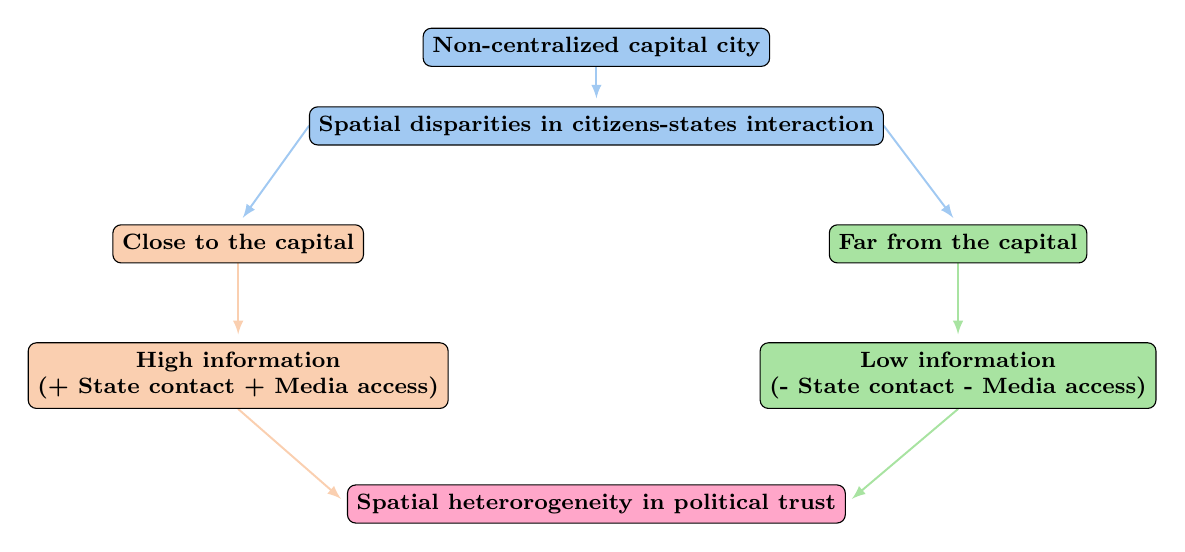
\begin{tikzpicture}
        \tikzset{
          node distance=5mm and 0mm,
          boite/.style={
            fill=blue!50!cyan!70,draw,align=center,
            font=\footnotesize\bfseries,text=black,
          },
          boite coins ronds/.style={boite,rounded corners=3pt},
          boite circulaire/.style={boite,circle},
          fleche/.style={
            line cap=round,-latex,line width=0.25mm,
            draw=blue!50!cyan!30,
          },
          grosse fleche/.style={fleche,line width=1mm},
          }
        \node[boite coins ronds, fill=babyblueeyes]  (a) {Non-centralized capital city};    
        \node[boite coins ronds, fill=babyblueeyes, below=of a]  (b) {Spatial disparities in citizens-states interaction};
        \node[boite coins ronds, fill=apricot, below left=1cm and -0.7cm of b] (c) {Close to the capital};
        \node[boite coins ronds, fill=grannysmithapple, below right=1cm and -0.7cm of b] (d) {Far from the capital};
        \node[boite coins ronds, fill=grannysmithapple, below=1cm of d] (f) {Low information\\(- State contact - Media access)};
        \node[boite coins ronds,fill=apricot, below = 1cm of c] (e) {High information\\(+ State contact + Media access)};
        \node[draw=none, fill=none] (dummy) at (0,-5) {}; % Create a dummy node at a specific position, not visible
        \node[boite coins ronds, fill=carnationpink] (g) at (0,-5.8) {Spatial heterorogeneity in political trust}; 
            
        \begin{scope}[on background layer]
            \draw[fleche,draw=babyblueeyes, shorten >=1mm]
            (a.south) -- (b.north) node[midway]{};  
            \draw[fleche,draw=babyblueeyes, shorten >=1mm]
            (b.west) -- (c.north) node[midway]{};
            \draw[fleche,draw=babyblueeyes, shorten >=1mm]
            (b.east) -- (d.north) node[midway]{};
            \draw[fleche,draw=apricot, shorten >=1mm]
            (c.south) -- (e.north) node[midway]{};
            \draw[fleche,draw=grannysmithapple, shorten >=1mm]
            (d.south) -- (f.north) node[midway]{};
            \draw[fleche,draw=apricot, shorten >=1mm]
            (e.south) -- (g.west)  node[midway]{};
            \draw[fleche,draw=grannysmithapple, shorten >=1mm]
            (f.south) -- (g.east)  node[midway]{};
            
        \end{scope}
      \end{tikzpicture}
    \end{frame}


    \begin{frame}{This paper}
        \centering
        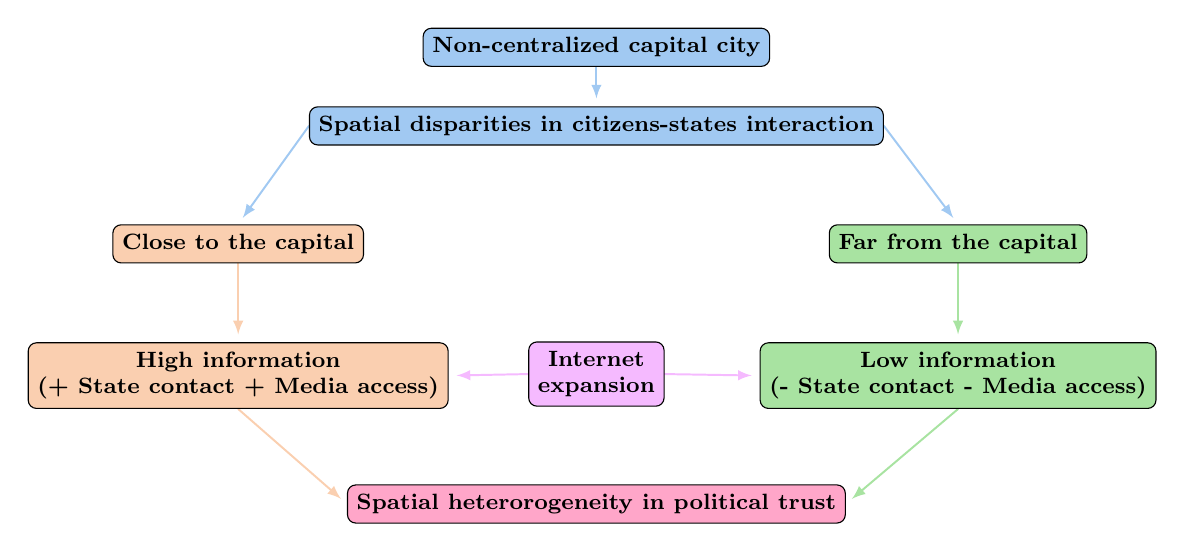
\begin{tikzpicture}
                \tikzset{
                  node distance=5mm and 0mm,
                  boite/.style={
                    fill=blue!50!cyan!70,draw,align=center,
                    font=\footnotesize\bfseries,text=black,
                  },
                  boite coins ronds/.style={boite,rounded corners=3pt},
                  boite circulaire/.style={boite,circle},
                  fleche/.style={
                    line cap=round,-latex,line width=0.25mm,
                    draw=blue!50!cyan!30,
                  },
                  grosse fleche/.style={fleche,line width=1mm},
                  }
                \node[boite coins ronds, fill=babyblueeyes]  (a) {Non-centralized capital city};    
                \node[boite coins ronds, fill=babyblueeyes, below=of a]  (b) {Spatial disparities in citizens-states interaction};
                \node[boite coins ronds, fill=apricot, below left=1cm and -0.7cm of b] (c) {Close to the capital};
                \node[boite coins ronds, fill=grannysmithapple, below right=1cm and -0.7cm of b] (d) {Far from the capital};
                \node[boite coins ronds, fill=grannysmithapple, below=1cm of d] (f) {Low information\\(- State contact - Media access)};
                \node[boite coins ronds,fill=apricot, below = 1cm of c] (e) {High information\\(+ State contact + Media access)};
                \node[boite coins ronds,fill=brilliantlavender] (dummy) at (0,-4.15) {Internet\\expansion}; % Create a dummy node at a specific position, not visible
                \node[boite coins ronds, fill=carnationpink] (g) at (0,-5.8){Spatial heterorogeneity in political trust}; 
                
                \begin{scope}[on background layer]
                    \draw[fleche,draw=babyblueeyes, shorten >=1mm]
                    (a.south) -- (b.north) node[midway]{};  
                    \draw[fleche,draw=babyblueeyes, shorten >=1mm]
                    (b.west) -- (c.north) node[midway]{};
                    \draw[fleche,draw=babyblueeyes, shorten >=1mm]
                    (b.east) -- (d.north) node[midway]{};
                    \draw[fleche,draw=apricot, shorten >=1mm]
                    (c.south) -- (e.north) node[midway]{};
                    \draw[fleche,draw=grannysmithapple, shorten >=1mm]
                    (d.south) -- (f.north) node[midway]{};
                    \draw[fleche,draw=apricot, shorten >=1mm]
                    (e.south) -- (g.west)  node[midway]{};
                    \draw[fleche,draw=grannysmithapple, shorten >=1mm]
                    (f.south) -- (g.east)  node[midway]{};
                    \draw[fleche,draw=brilliantlavender, shorten >=1mm]
                    (dummy.west) -- (e.east)  node[midway]{};
                    \draw[fleche,draw=brilliantlavender, shorten >=1mm]
                    (dummy.east) -- (f.west)  node[midway]{};
                    
                \end{scope}
              \end{tikzpicture}
            \end{frame}




            %\begin{frame}{This paper}

                %\begin{itemize}
                    %\item Economic theory suggest that better information leads to more efficient outcomes in political institutions \textcolor{gray}{\textit{Besley and Burgess, 2002;
                    %Banerjee et al., 2011; Fujiwara and Wantchekon, 2013; Larreguy et al., 2020}} \vfill
                    %\item We document a spatial pattern in Sub-Saharan Africa:\\ \vfill
                    %\vspace{1em}
                    %\begin{center} Citizens living in remote areas have \textcolor{rougeprez}{\textbf{limited exposure to state institutions}} and \textcolor{rougeprez}{\textbf{reduced access to information infrastructure}} but they report \textcolor[rgb]{0.0,0.6,0.0}{\textbf{higher trust in state institutions}} relative to those near capitals \vfill
                    %\end{center}
                %\end{itemize}
            %\hspace{2.5em}$\Rightarrow$ \textit{Uninformed trust}
            %\begin{itemize}
                %\item Internet coverage reduces spatial disparities in political trust
            %\end{itemize}
            %\end{frame}

            %\begin{frame}{This paper}
             %   \centering The extent to which this potential is realized likely depends on several important scope conditions \vfill  \pause
             %   \begin{itemize}\setlength\itemsep{1em}
              %      \item Regional and ethnic favoritism from ruling governments \textcolor{gray}{\textit{Franck and Rainer, 2012;
              %      Hodler and Raschky, 2014; Kramon and Posner, 2016; De Luca et al., 2018}} \vfill  \pause
              %      \item Threatened governments may try to capture the functioning of these new information flows or the deployment of its infrastructure to
              %      preserve their advantages \textcolor{gray}{\textit{Chen and Xu, 2017; Morozov, 2012}} \vfill  \pause
              %      \item The quality and reliability of the information; if mobile
              %      internet facilitates misinformation and manipulation \textcolor{gray}{\textit{Cariolle et al., 2024; Van Zoonen et al., 2024}}, it could actually undermine rather than
              %      strengthen accountability linkages
              %  \end{itemize}    
           % \end{frame}
            

            \begin{frame}{Empirical strategy overview}    
                \centering Combine Afrobarometer geocoded surveys data across 20 Sub-Saharan countries
between 2011-2021, with GSMA digital maps of mobile internet coverage\\\vfill
\vspace{1em}
                \centering We examine \textbf{(1)} spatial disparities in political trust and \textbf{(2)} how mobile internet access expansion may affect these differences \vfill  \pause
                \vspace{1em}
                \setbeamertemplate{enumerate items}[default]
                \begin{enumerate}
                    \item Effect of capital city distance on political trust: \textcolor{rougeprez}{\textbf{Border
                    discontinuity design}} \vfill
                    \begin{itemize}
                        \item Colonial boundaries - which became modern national borders
                        - that arbitrarily divided historical ethnic homelands \textcolor{gray}{\textit{Michalopoulos and Papaioannou, 2014; Provenzano, 2024}}\vfill
                        \item Sharp variations in citizens’
                        distances from their respective national capital\vfill  \pause
                    \end{itemize}

                    \item Internet coverage effect: \textcolor{rougeprez}{\textbf{Instrumental variable}}\vfill

                    \begin{itemize}
                    \item Instrument for internet coverage using lightning strike
                    patterns \textcolor{gray}{\textit{Manacorda and Tesei, 2020; Guriev et al., 2021}}\vfill
                    \item Areas with frequent lightning strikes have
                    higher costs for internet infrastructure deployment and maintenance, while these weather
                    patterns are plausibly exogenous to political trust\vfill
                \end{itemize}

                \end{enumerate}
            \end{frame}

            
\begin{frame}{Main results}

    \setbeamertemplate{enumerate items}[default]
    \begin{enumerate}\setlength\itemsep{0.5em}
        \item \definecolor{rougeprez}{RGB}{158,27,50}\textcolor{rougeprez}{\textbf{Distance from the capital effect}}\\
        \begin{itemize}
            \item Remote areas (↑ distance) show a 27\% higher political trust relative to the unconditional standard deviation
            \begin{itemize}
                \item Robust to border discontinuity design using national boundaries overlapping ethnic areas  \pause
            \end{itemize}
        \end{itemize}
        \item \definecolor{rougeprez}{RGB}{158,27,50}\textcolor{rougeprez}{\textbf{Internet coverage effect}}\\
        \begin{itemize}
            \item Internet coverage reduces spatial disparities in political trust
            \begin{itemize}
                \item Strong negative interaction between distance and internet coverage
                \item Robust to IV strategy using lightning strike patterns  \pause
            \end{itemize}
        \end{itemize}
        \item \definecolor{rougeprez}{RGB}{158,27,50}\textcolor{rougeprez}{\textbf{Political accountability}}\\
            \begin{itemize}
                \item Citizens with internet access in remote areas are more critical of the economy
                \item They are more willing to sanction the ruling party through voting  \pause
            \end{itemize}
        \item  \definecolor{rougeprez}{RGB}{158,27,50}\textcolor{rougeprez}{\textbf{Information censorship}}
        \begin{itemize}
            \item Stronger effect where the government controls the traditional media and institutions
            \item Major source of news when no other independent information are available  \pause
        \end{itemize}
        
    \end{enumerate}
    \vspace{0.5em}
    \begin{center}
        \textbf{Internet access facilitates the shift from \textit{uninformed trust} to active democratic engagement, particularly in previously isolated areas}
    \end{center}
\end{frame}


\begin{frame}{Literature contribution}

    \begin{itemize}\setlength\itemsep{1em}
        \item Geography of trust \vfill
        \begin{itemize}
            \item Distance from administrative centers \textcolor{gray}{\textit{Brinkerhoff et al. 2018; Bland et al., 2023; Li, 2004}} \vfill
            \item Higher institutional trust in rural area \textcolor{gray}{\textit{McKay et al., 2023; Li, 2004}} \vfill
        \end{itemize}
        \textcolor{rougeprez}{\textbf{$\rightarrow$ Distance shapes citizens’ political trust}}\vfill
        \item Political economy of the capital city \vfill
        \begin{itemize}
            \item National institutions’ reach \textcolor{gray}{\textit{Herbst, 2000; Michalopoulos and Papaioannou, 2014}} \vfill
            \item Democratic accountability \textcolor{gray}{\textit{Provenzano, 2024; Gottlieb, 2016}} \vfill
            \item State capacity \textcolor{gray}{\textit{Pierskalla et al., 2017; Müller-Crepon, 2023}}  \vfill
        \end{itemize}
        \textcolor{rougeprez}{$\rightarrow$ \textbf{Strategic placement affects patterns of political trust and democratic engagement}}\vfill    

        \item Internet role in accountability and governance information\vfill
        \begin{itemize}
            \item Governance satisfaction \textcolor{gray}{\textit{Guriev et al., 2021; Cariolle et al., 2024; Miner, 2015}} \vfill
            \item Electoral accountability \textcolor{gray}{\textit{Donati, 2023; Chong et al., 2015}} \vfill
        \end{itemize}
        \textcolor{rougeprez}{$\rightarrow$ \textbf{Connectivity reshapes spatial patterns of accountability}}\vfill
    \end{itemize}
    \end{frame}
    

\begin{frame}{Data}
    
    \begin{columns}
    \begin{column}{0.5\textwidth}
    \begin{itemize}\setlength\itemsep{1em}
    \item Afrobarometer surveys accross 20 Sub-Saharan countries: rounds 5 to 8 (2011-2021)
    \vspace{0.05cm}
    \begin{itemize}\setlength\itemsep{0.05cm}
        \item Geolocated information on public opinion, media consumption and demographic characteristics at the individual level
        \item Distance from the capital city
    \end{itemize}
    \item Collins Bartholomew’s Mobile Coverage Explorer: 2G/3G network coverage (2011-2021)
    \begin{itemize}\setlength\itemsep{0.05cm}
        \vspace{0.05cm}
        \item 1×1-kilometer binary grid cells
        \item Regional level mean coverage
        \item Weighted by UN-adjusted population density grid cells
    \end{itemize}
    %\item Other sources for controls: V-DEM, World Bank, Africa Integrity Indicators...
    \end{itemize}
    
    \end{column}
    \begin{column}{0.5\textwidth}
    
    \begin{figure}
        \centering
        \caption{Country Sample and Capital Cities}
        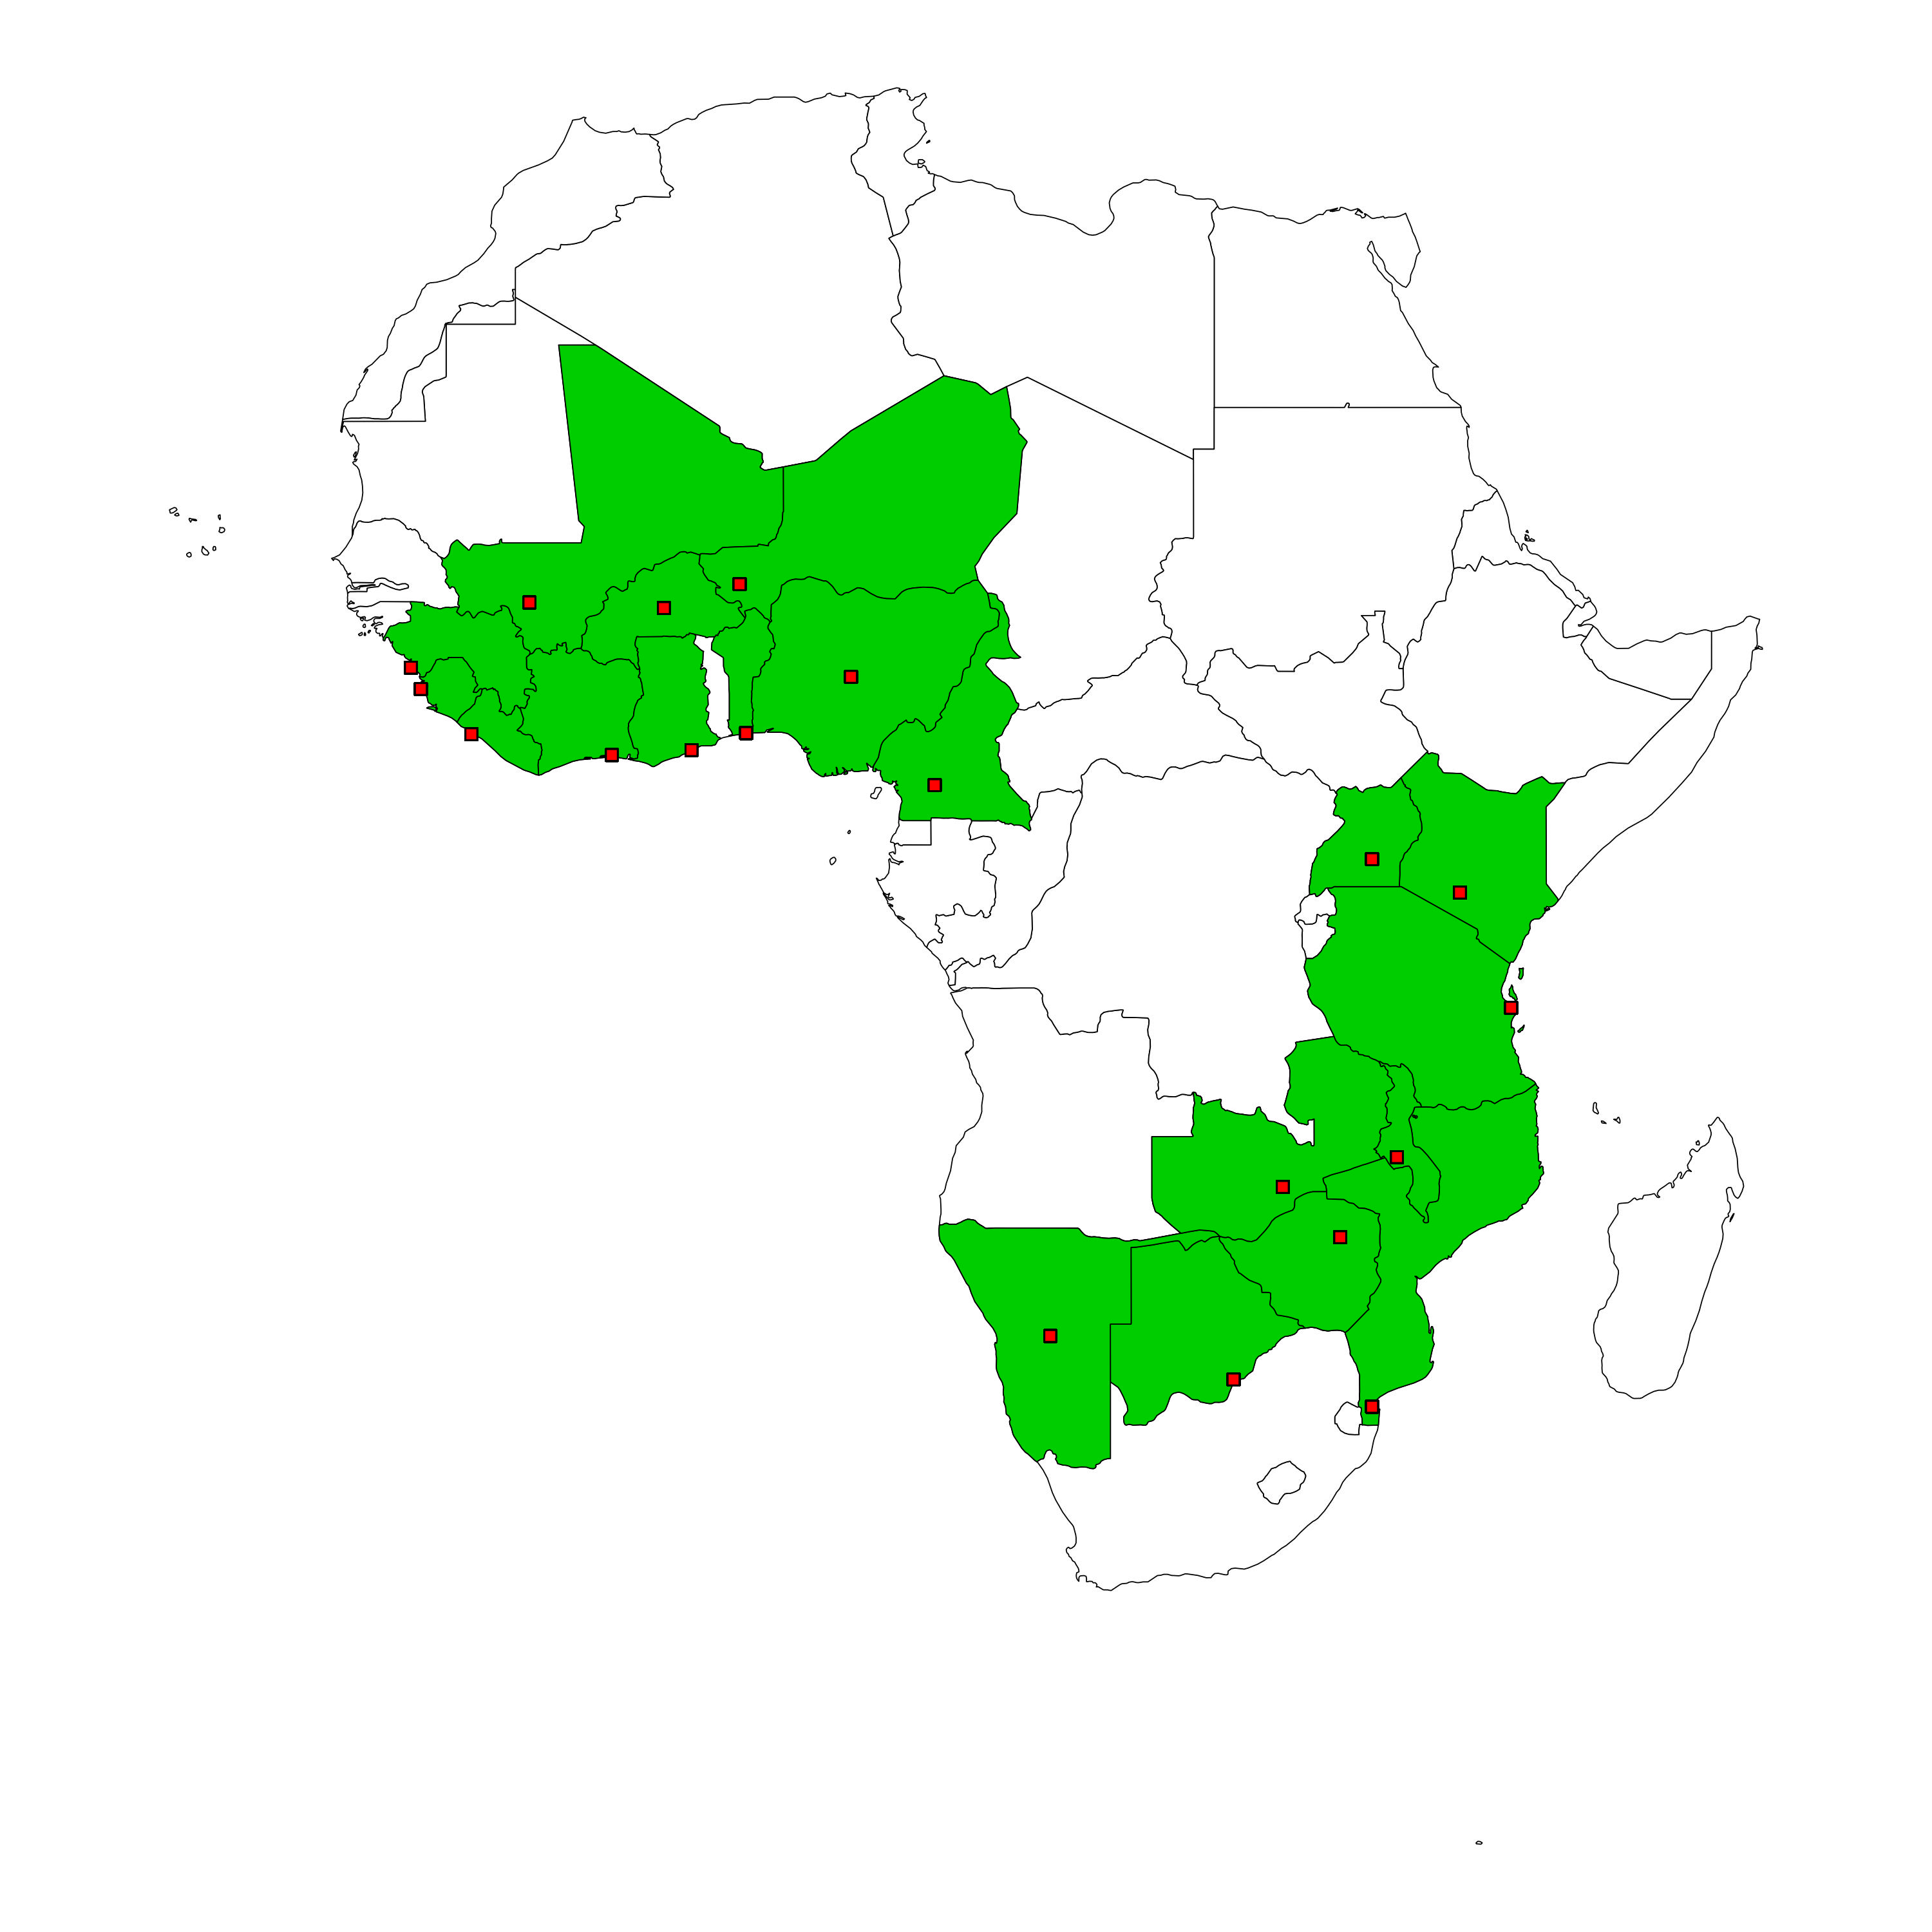
\includegraphics[width=6cm]{obs_map.jpg}
    \end{figure}
    \end{column}
        \end{columns}
    \end{frame}

\begin{frame}{Empirical strategy - Spatial disparities in political trust}
    \centering \textbf{Effect of distance from the capital city on political trust}\vspace{1em}
        \begin{equation}
        trust_{ict} = \beta_{0} + \beta_{1}distance_{ict} + \gamma X^{'}_{ir} + \mu_{ct} + \varepsilon_{ict}
        \end{equation}
        \begin{itemize}
            \item $trust_{ict}$: Average trust in parliament and president (0-3 scale)\vfill
            \item $distance_{ict}$: Relative distance measure (0-1 scale)\\
            \vspace{0.1cm}
            $\rightarrow{}$ \textcolor{gray}{\textit{Michalopoulos and Papaioannou, 2014}}\vfill
            \item $X^{'}_{ir}$: Set of individual and regional controls\vfill
            \item $\mu_{ct}$: Country $\times$ round fixed effects\vfill
            \item $\epsilon_{ict}$: Error term\vfill
            \item Robust standard errors clustered at the region x round level
        \end{itemize}
\end{frame}

\begin{frame}{Empirical strategy - Spatial disparities in political trust}

    \centering \textcolor{rougeprez}{\textbf{Border discontinuity design}} \vfill
    \begin{itemize}\setlength\itemsep{1em}
            \item Colonial boundaries - which became modern national borders
            - that arbitrarily divided historical ethnic homelands  \textcolor{gray}{\textit{Michalopoulos and Papaioannou, 2014; Provenzano, 2024}}\vfill
            \item These arbitrary divisions created
            quasi-random national affiliations in border regions, generating sharp variations in citizens’
            distances from their respective national capital \vfill
            \item Compare individuals from the same ethnic group who, due to colonial boundaries, live at different distances
            from their capital cities \vfill
        \end{itemize}
\end{frame}

\begin{frame}{Empirical strategy - Spatial disparities in political trust}
    \begin{figure}
        \centering
        \caption{Historical Ethnic Areas and Contemporary National Boundaries}
        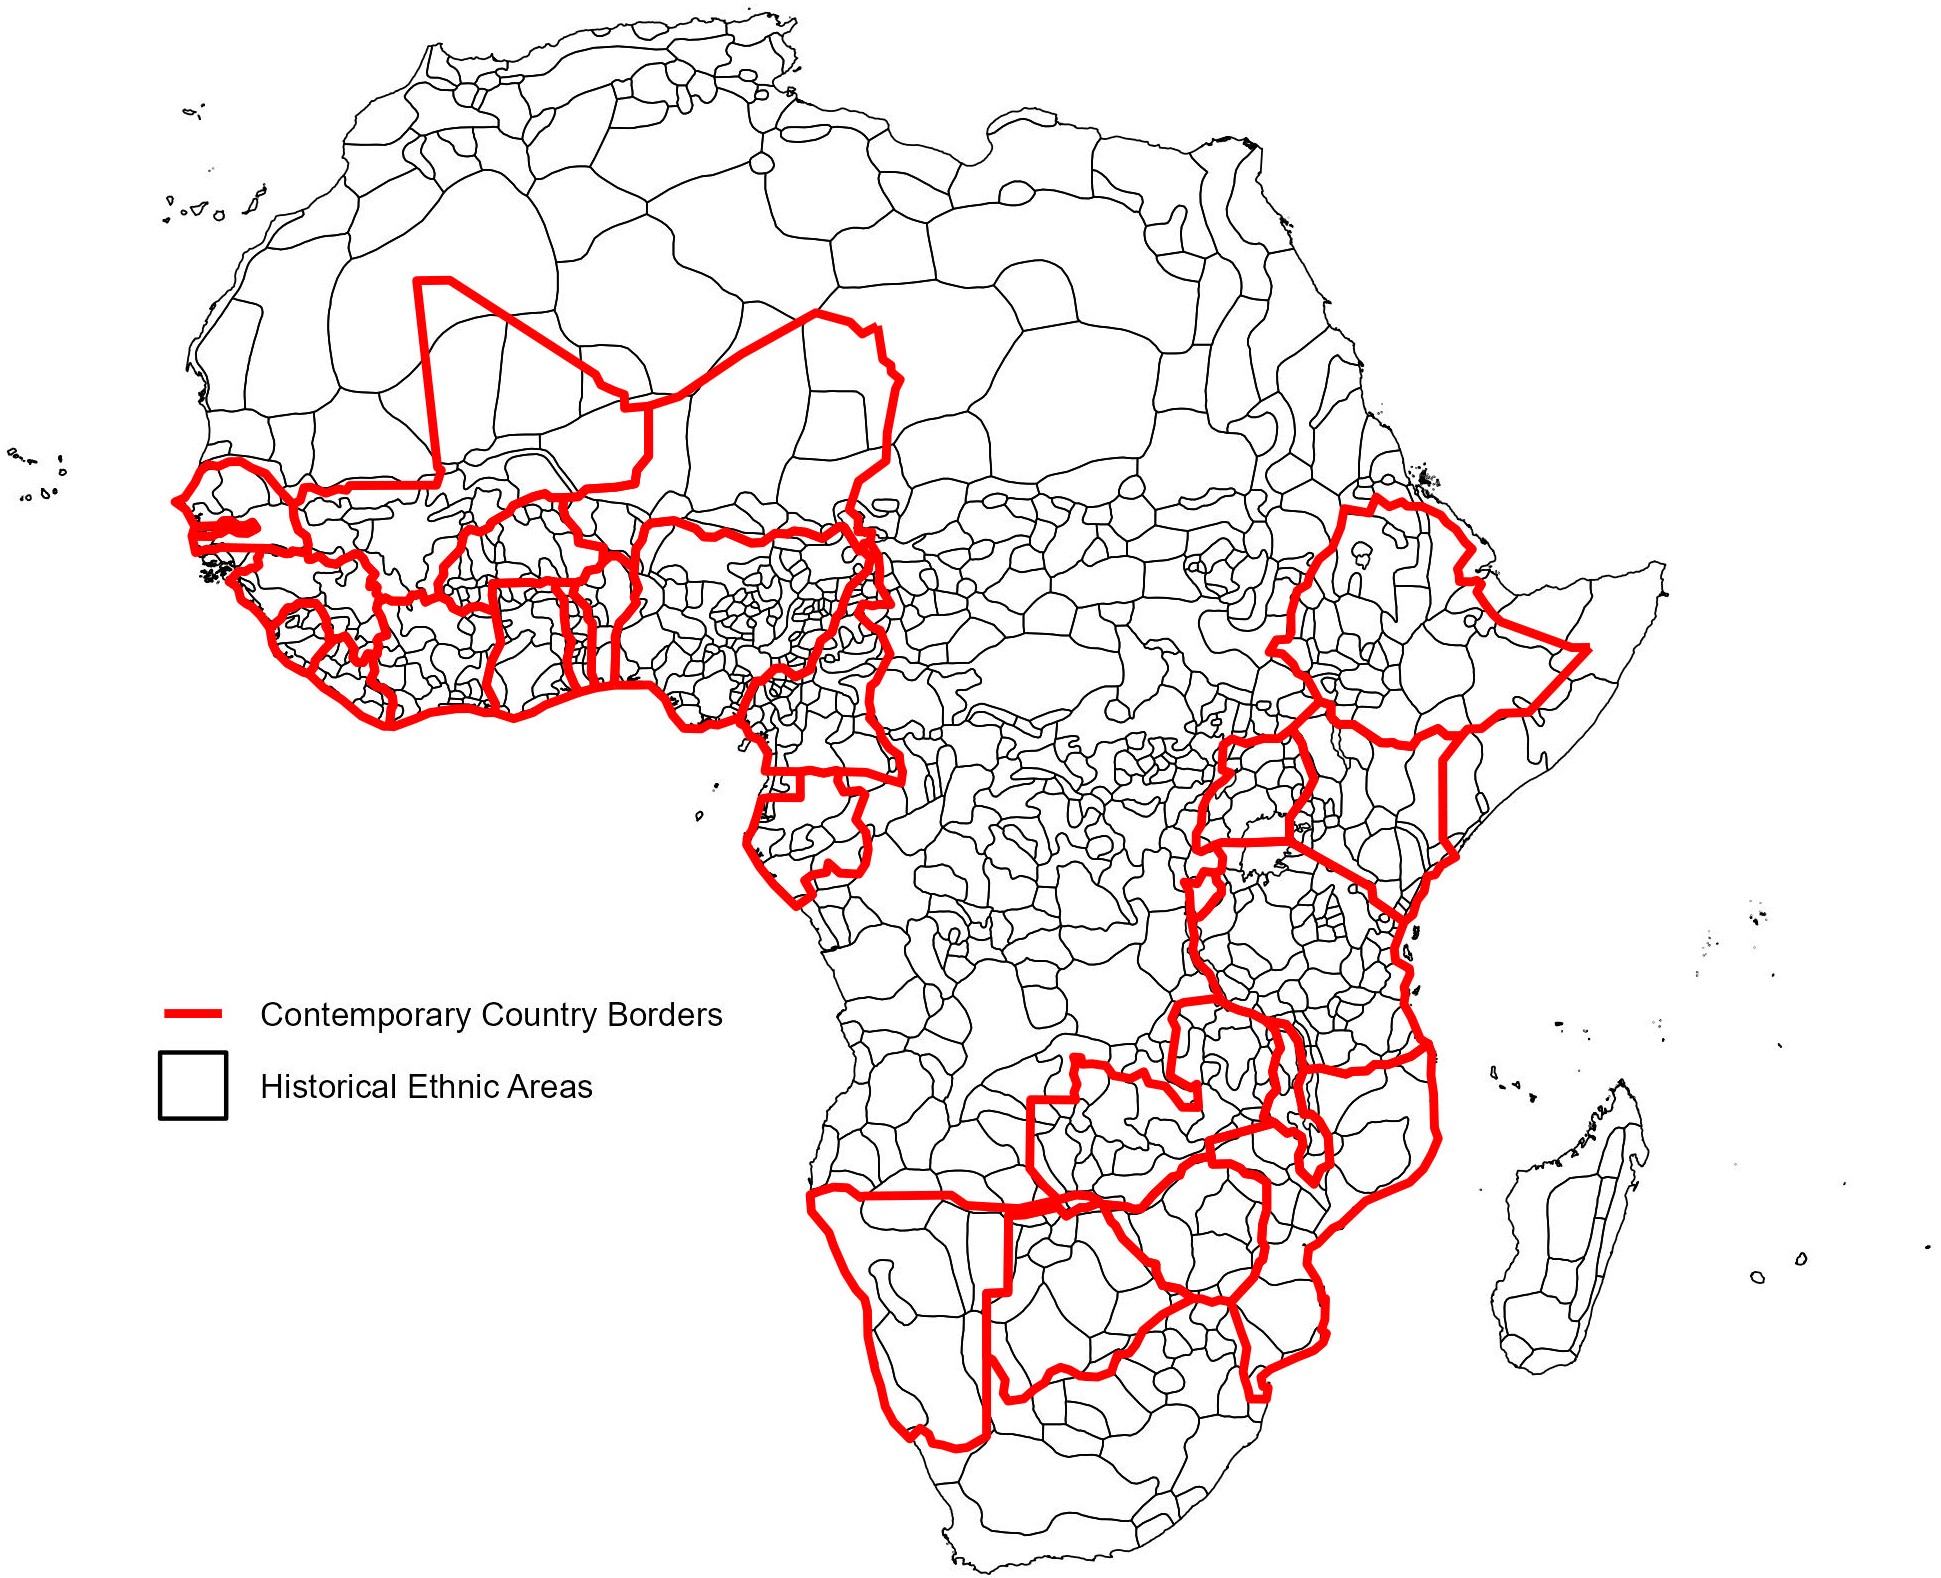
\includegraphics[width=8cm]{murdock_map.jpg}
    \end{figure}
    
\end{frame}


\begin{frame}{Empirical strategy - Spatial disparities in political trust}

    \begin{figure}
        \centering
        \caption{Exemple: Dendi Ethnic Group}
        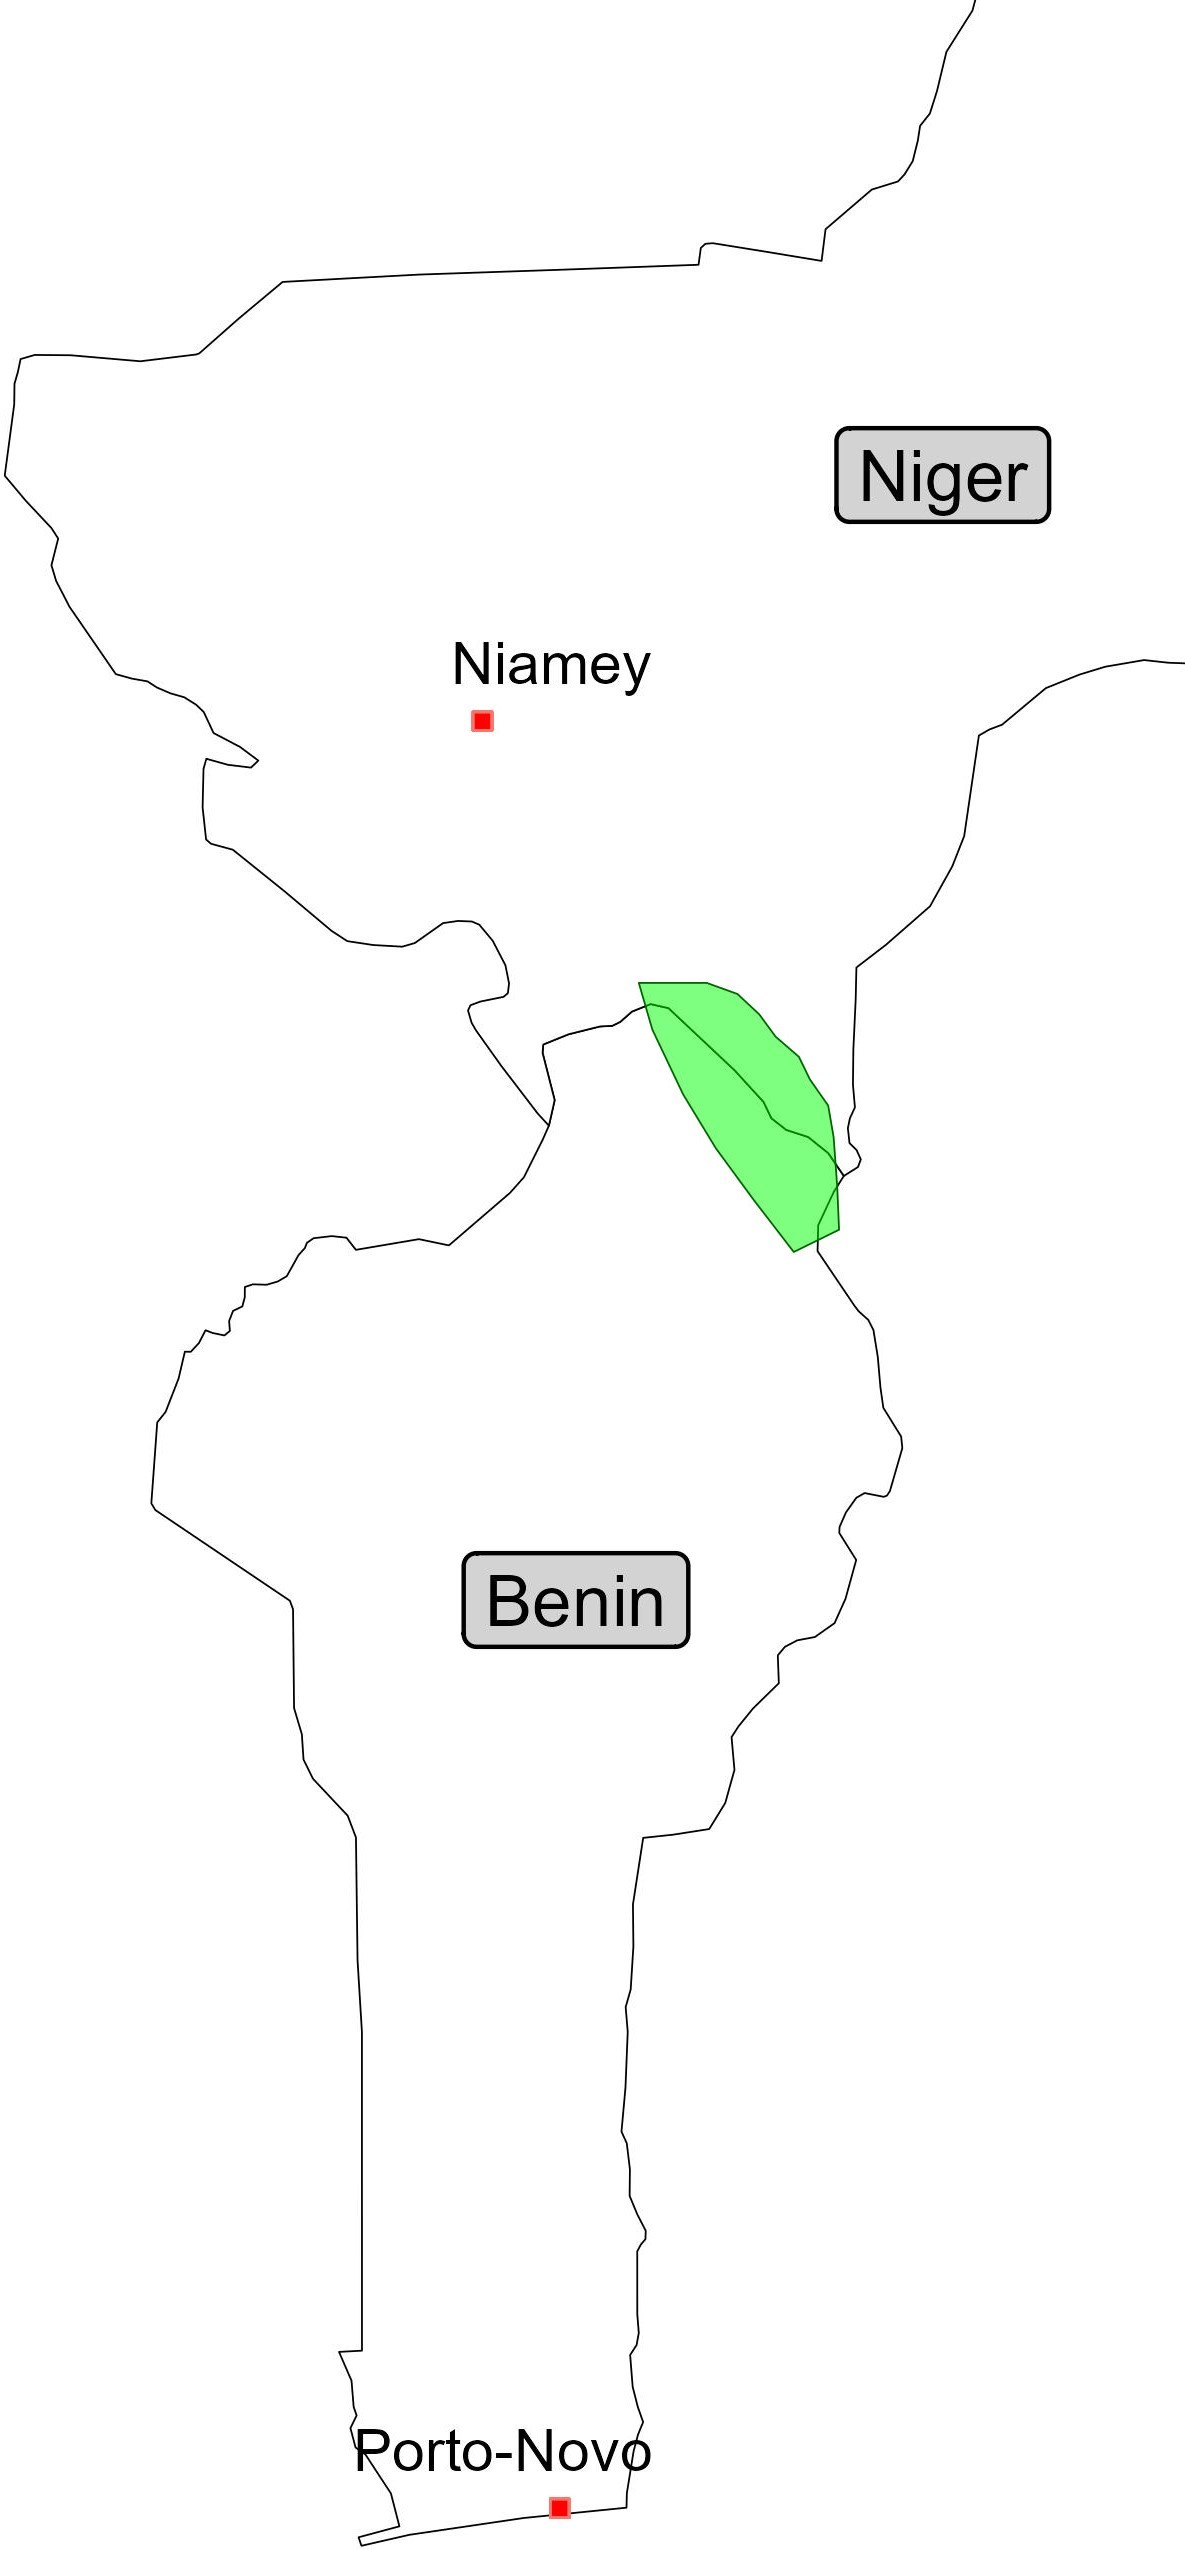
\includegraphics[width=2.8cm]{bdd_map.jpg}
    \end{figure}

\begin{equation}
trust_{ict}=\beta_{0}+\beta_{1}distance_{ict}+\gamma X^{'}_{ir}+\textcolor[rgb]{0.0,0.6,0.0}{\mathbf{\nu_{e}}}+\mu_{ct}+\varepsilon_{ict}
\end{equation}

\end{frame}


\begin{frame}{Empirical strategy - Spatial disparities in political trust}
    \centering \textcolor{rougeprez}{\textbf{Identification assumptions}}\vfill
    \setbeamertemplate{enumerate items}[default]
    \begin{enumerate}
        \item Two individuals living in the same historical ethnic region share similar geographical, social, and historical traits, except for their distance from the capitals\vfill
        \item The differences observed on either side of the country border are not attributable to institutional differences\vfill
        
\begin{equation}
    trust_{ict}=\beta_{0}+\beta_{1}distance_{ict}+\gamma X^{'}_{ir}+ \textcolor[rgb]{0.0,0.6,0.0}{\theta Z^{'}_{ct}} + \textcolor[rgb]{0.0,0.6,0.0}{\mathbf{\nu_{e}}}+\textcolor[rgb]{0.0,0.6,0.0}{\lambda_{t}}+\varepsilon_{ict}
    \end{equation}
            
    \end{enumerate}
\end{frame}







\begin{frame}{Distance increases political trust}


    \begin{table}[H]
        \sffamily
        \caption{{Effect of distance from the capital on political trust}}
        \centering
        %\footnotesize
        \resizebox{8cm}{!}{
        \begin{tabular}{@{\extracolsep{5pt}} l c c c c}
        \\
        \toprule
        \toprule
        &  \multicolumn{4}{c}{{OLS}}  \\
        \cmidrule(r){2-5}
        &  \multicolumn{4}{c}{{Political trust}}  \\
        \cmidrule(r){2-5}
        & \multicolumn{2}{c}{{Base sample}} & \multicolumn{2}{c}{{Border sample}}\\
            \cmidrule(r){2-3}
            \cmidrule(r){4-5}
            & \multicolumn{1}{c}{{(1)}} &  \multicolumn{1}{c}{{(2)}}  & \multicolumn{1}{c}{{(3)}} &  \multicolumn{1}{c}{{(4)}}\\
         \midrule
      
         Distance from the capital&       0.284***&       0.270***&       0.681***&       0.397* \\
         \medskip
         &      (0.04)   &      (0.03)   &      (0.16)   &      (0.21)  \\
         \midrule
         \smallskip
        Individual \& regional controls  & Yes & Yes & Yes & Yes  \\
        \smallskip
        Country controls & Yes& No& Yes& No\\
        \smallskip
        Round FE & Yes & No& Yes & No\\
        \smallskip
        Country X Round FE       & No & Yes& No & Yes\\
        \smallskip
        Ethnic homeland FE & No & No & Yes& Yes\\
        \smallskip
        Observations           & 98,235   &       98,235   &        4,189   &        4,189   \\
        Adjusted-R$^2$        &       0.158   &       0.197   &       0.159   &       0.189   \\
    
                              \bottomrule
        \multicolumn{5}{p{12.5cm}}{\footnotesize \emph{Notes}: The border sample includes individuals residing within a 20-kilometer buffer around a country border that overlaps with a historical ethnic homeland, as defined by Murdock (1959). Robust standard errors clustered at the region x round level  for the base sample and ethnic homeland x region x round level for the border sample are in parentheses. The set of individual controls
        includes values of: normalized distance from the largest non-capital city, age, age squared, sex,
        education, employment status, rural/urban situation, personal economic conditions perception, ethnic discrimination, interest in politics, TV news consumption, radio news consumption, newspaper news consumption. The set of regional controls includes values of: nighttime light, population density, region area, president birthplace dummy. The set of country controls includes: log(GDP.p.c.), log(area), V-Dem Polyarchy index, World Bank corruption index, political regime type, colonial origin. *** / ** / * represent significance at the 0.01 / 0.05 / 0.10 levels, respectively.}
        \end{tabular}
        }
        \end{table}
    \end{frame}

\begin{frame}{Distance increases political trust}

\begin{figure}
    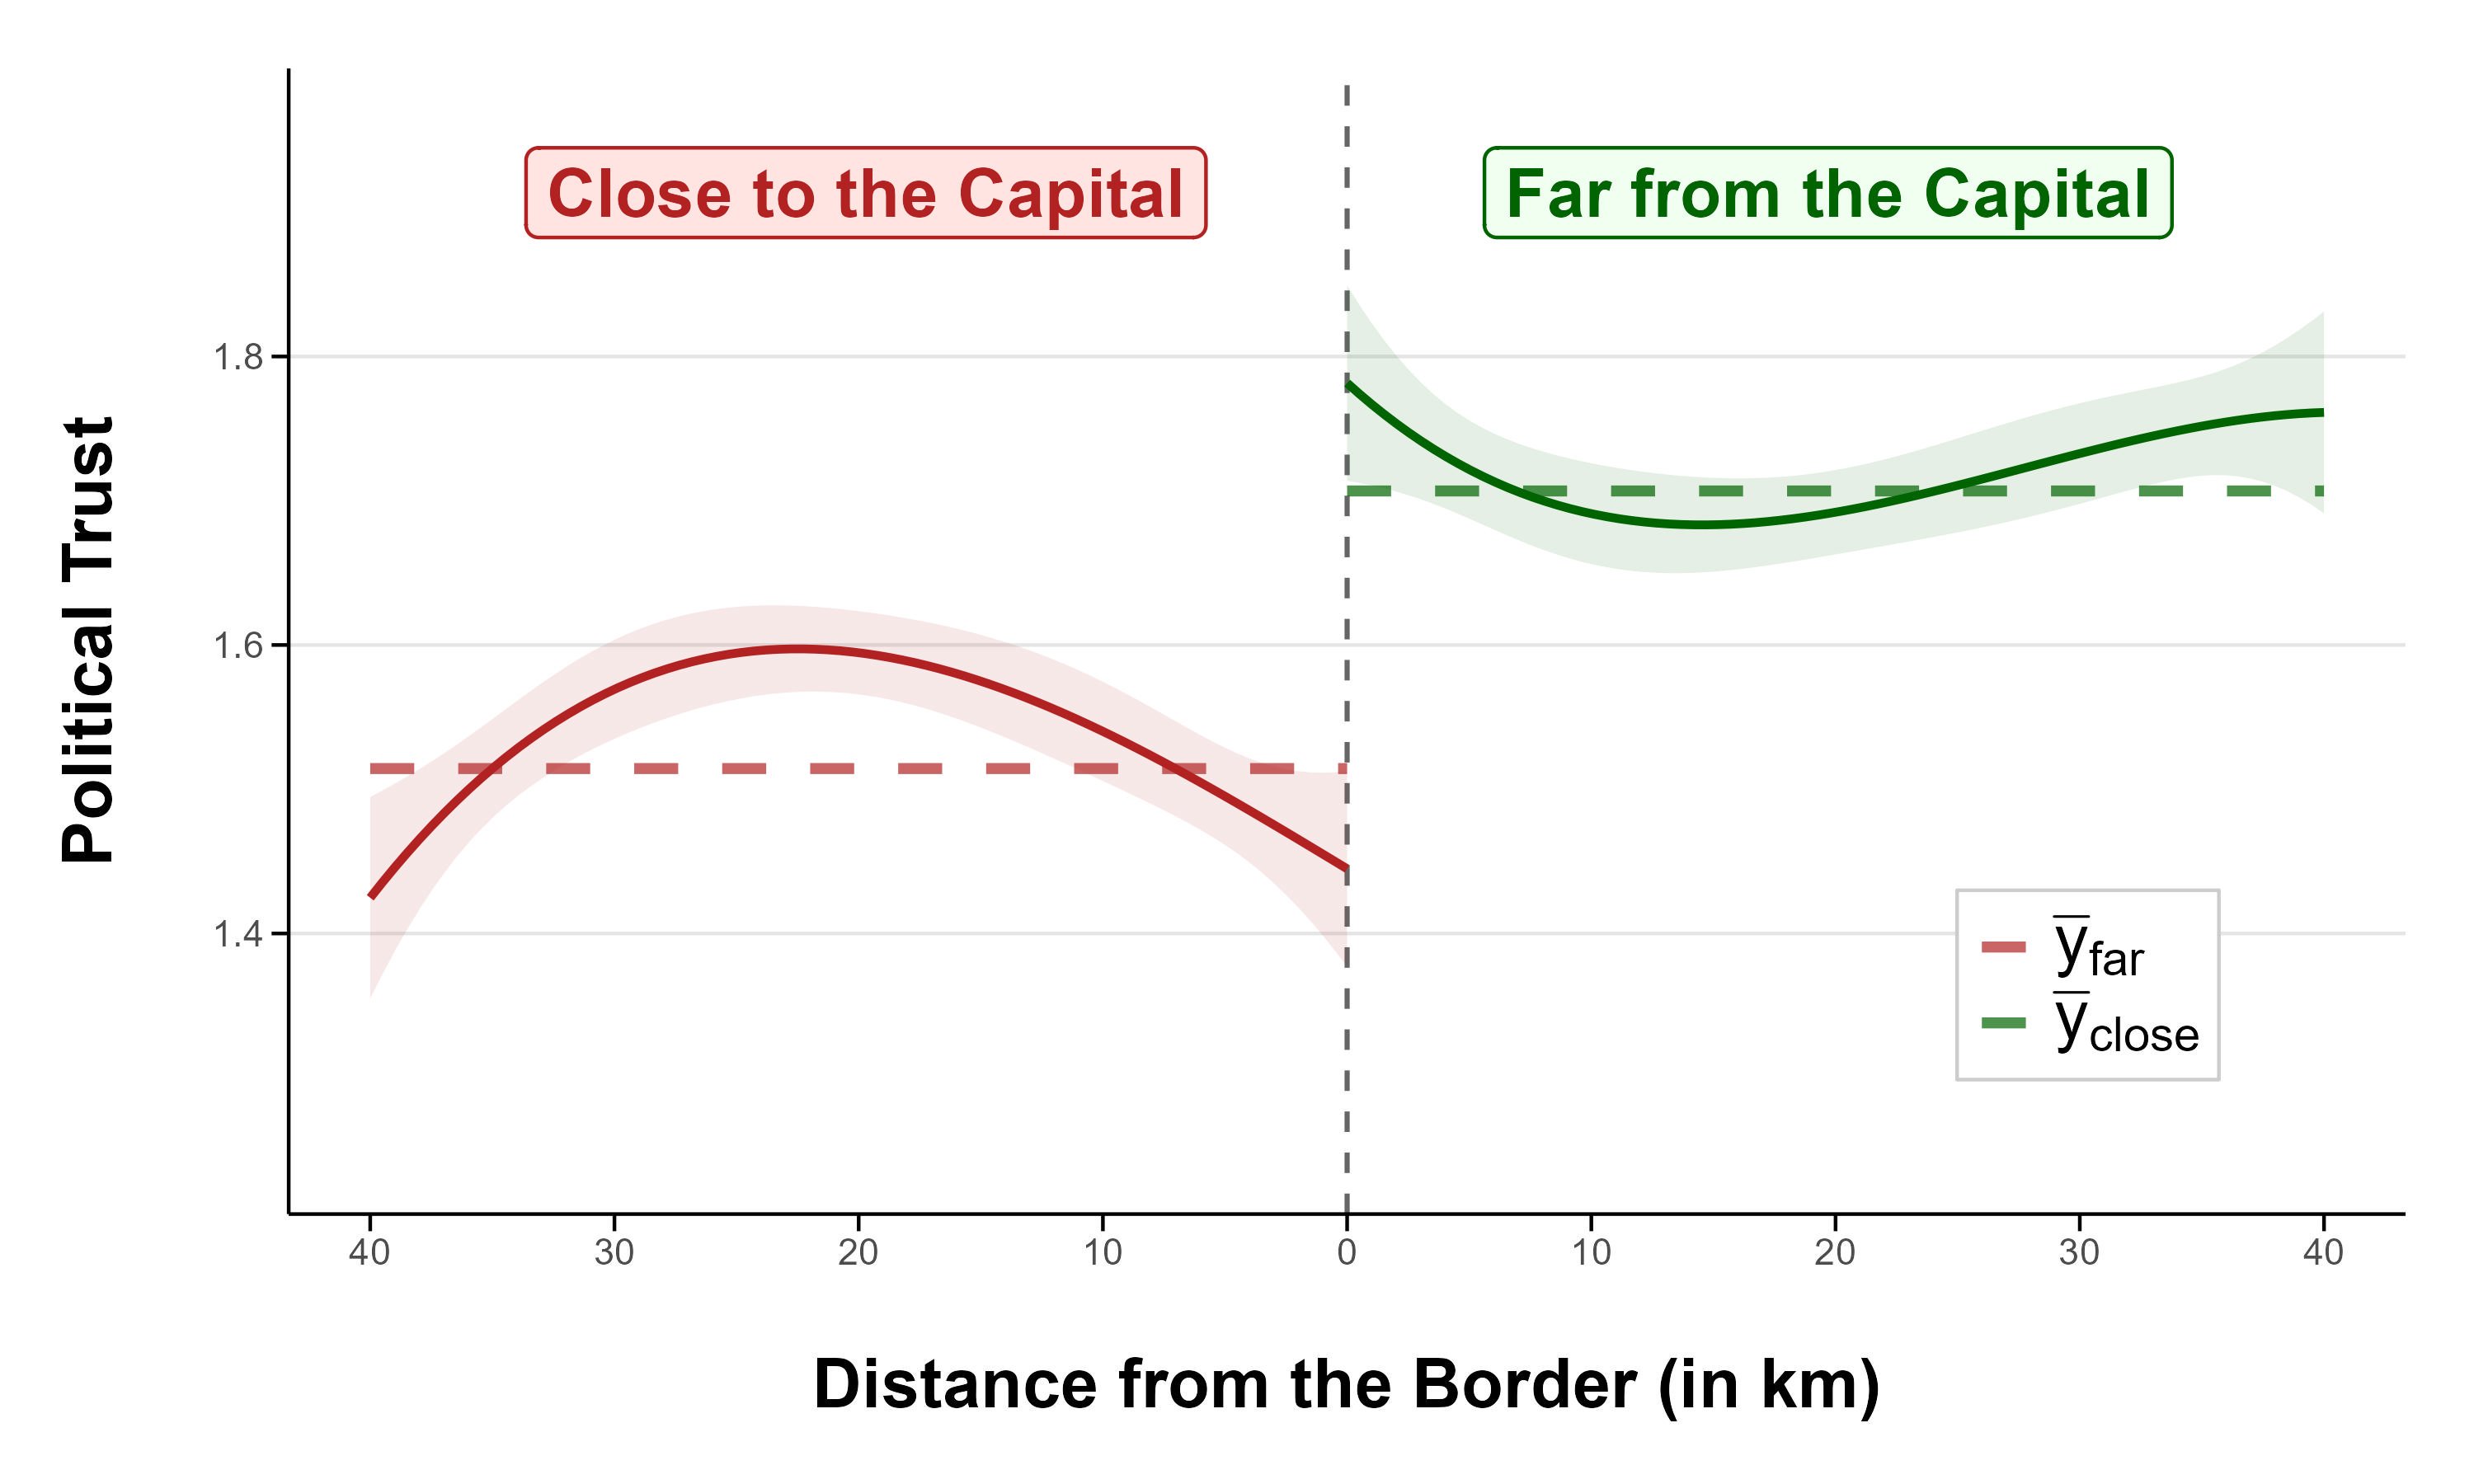
\includegraphics[scale=0.1]{C:/Users/Redha CHABA/Documents/Working paper/trust/script/plots/discontinuity/discontinuity.jpg}
    \caption{Border discontinuity - \textit{Based on regression estimates from (3) of Table 1}}
\end{figure}

\end{frame}


\begin{frame}{{\fontsize{13}{12}\selectfont
    Empirical strategy - Internet coverage and spatial disparities}}
\centering \textcolor{rougeprez}{\textbf{Effect of internet coverage on political trust by distance}}\vspace{1em}

\begin{equation}
    \fontsize{8}{10}\selectfont
\begin{split}
trust_{ict} = & \beta_{0} + \beta_{1} distance_{ict} + \beta_{2} \textcolor{red}{\textbf{internet\_coverage}_{ict}} + \beta_{3} \textcolor{red}{\textbf{distance} \times \textbf{internet\_coverage}_{ict}} \\
& + \gamma X^{'}_{ir} + \mu_{ct}+ \varepsilon_{ict}
\end{split}
\end{equation}\vspace{1em}

\noindent
{\fontsize{9}{12}\selectfont
\textcolor{red}{\textbf{internet\_coverage}$_{ict}$:} Regional average of internet coverage weighted by population density \textcolor{gray}{\textit{Guriev et al., 2021, Cariolle and Carroll, 2024}}
}
\vfill

\begin{itemize}
    \item \textcolor{red}{\textbf{Reverse causality:}} Areas with higher political trust might experience less deployment of internet infrastructure
\end{itemize}
\end{frame}

\begin{frame}{{\fontsize{13}{12}\selectfont
    Empirical strategy - Internet coverage and spatial disparities}}
    \begin{figure}
        \centering
        \caption{Example: Benin Lightning Strikes and Internet Coverage}
        
        \begin{subfigure}{0.45\textwidth}
            \centering
            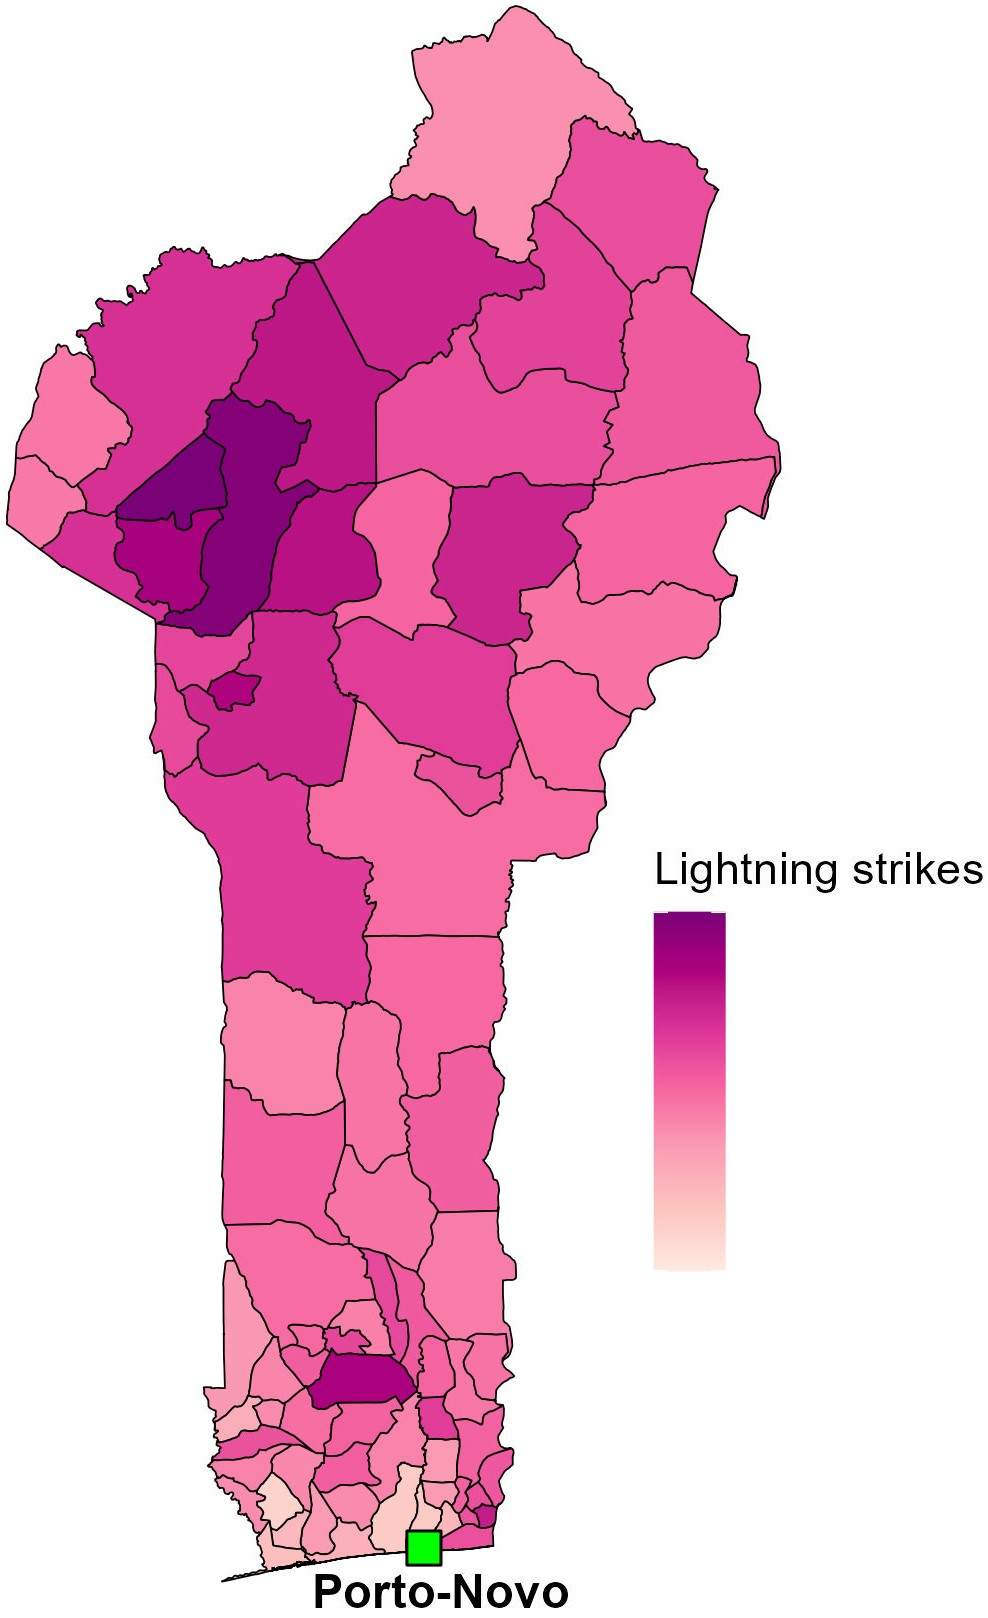
\includegraphics[width=3.8cm]{lightning_strikes.jpg}
            \caption{Lightning strikes}
        \end{subfigure}
        \hspace{0.02\textwidth}
        \begin{subfigure}{0.45\textwidth}
            \centering
            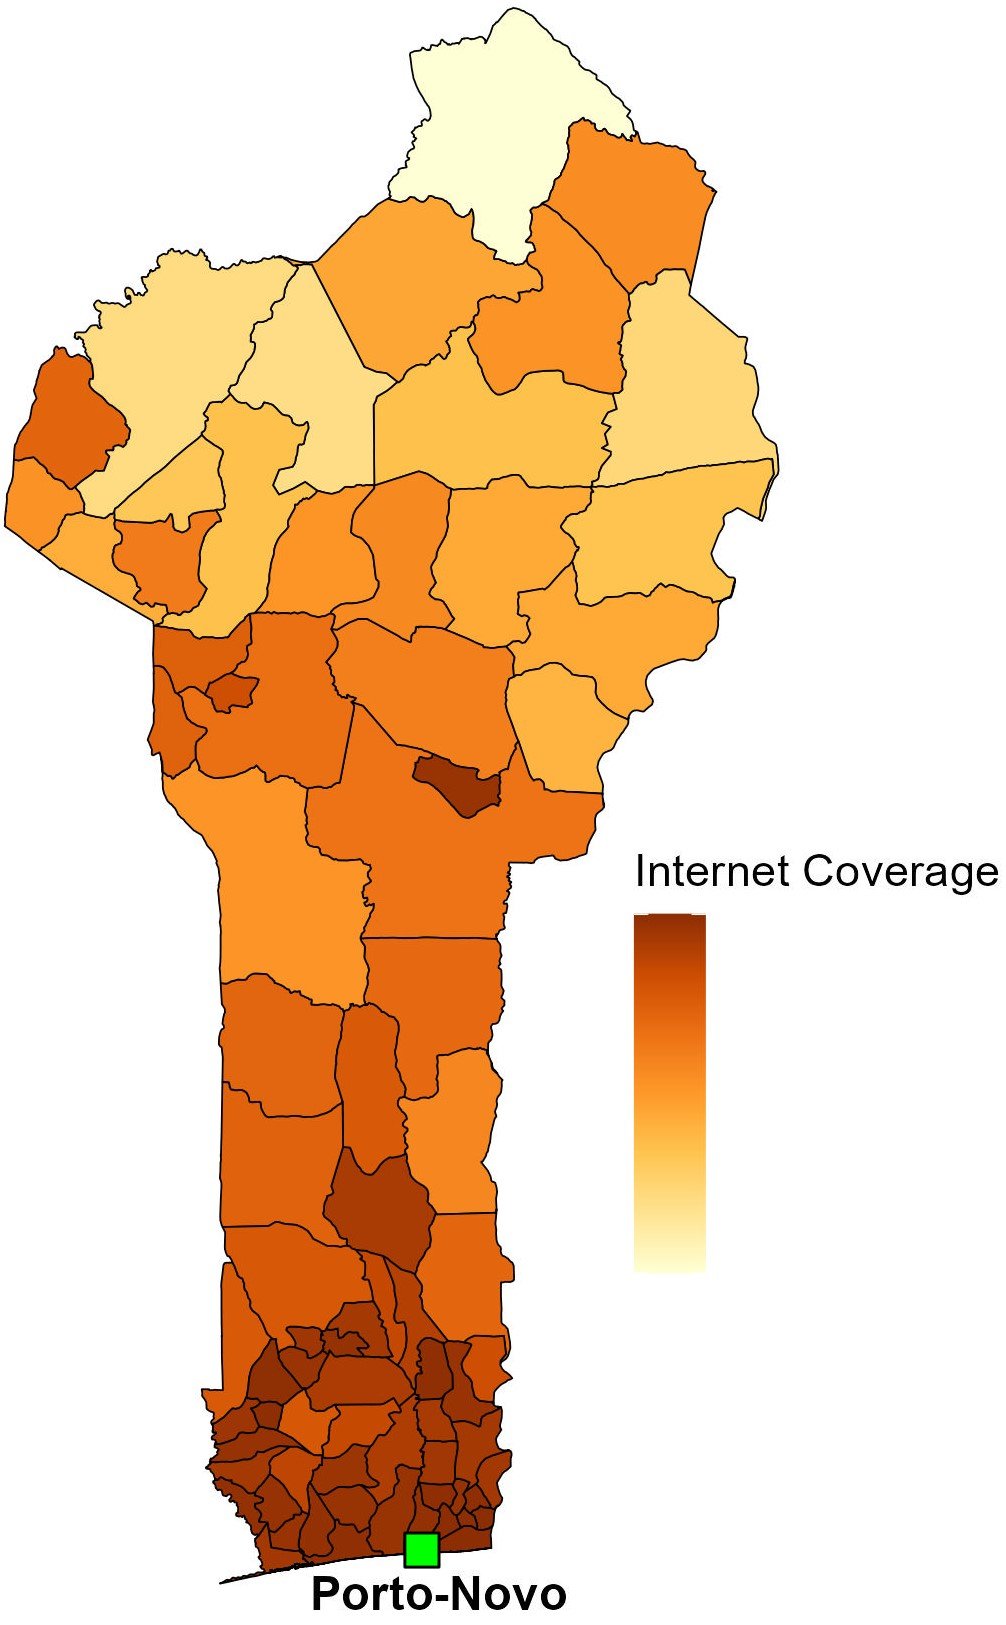
\includegraphics[width=3.8cm]{internet_coverage_w8.jpg}
            \caption{Internet coverage (2019-2021)}
        \end{subfigure}
        
    \end{figure}
\end{frame}

\begin{frame}{{\fontsize{13}{12}\selectfont
    Empirical strategy - Internet coverage and spatial disparities}}    
    \centering \textcolor{rougeprez}{\textbf{Lightning strikes instrument}}
    \vspace{1.5em}
    \begin{itemize}\setlength\itemsep{1em}
        \item Instrument internet coverage
        using regional lightning strike patterns \textcolor{gray}{\textit{Manacorda and Tesei, 2020; Guriev
                et al., 2021; Cariolle and Carolle, 2024}}\vfill
        \item Areas with frequent lightning strikes face higher infrastructure deployment and maintenance costs, while these weather patterns
                are plausibly exogenous to political trust\vfill
        \item Average daily lightning strikes at the regional level using VHRFC data over 1998-2013, weighted by regional population density\vfill
    \end{itemize}
    \vspace{1em}

\centering \textcolor{rougeprez}{\textbf{Geographical instrument $\rightarrow$ focus on the base sample}}
\end{frame}

\begin{frame}{{\fontsize{13}{12}\selectfont
    Empirical strategy - Internet coverage and spatial disparities}}
    \centering \textbf{First-stage}

    \begin{equation}
        \begin{split}
            \textcolor{red}{\textbf{internet\_coverage}_{ict}} = & \beta_{0} + 
            \beta_{1} \textcolor[rgb]{0.0,0.6,0.0}{\textbf{lightning\_strike}_{r} \times t} + \gamma X^{'}_{ir} \\
            & \quad + \mu_{ct}+ v_{ict}
        \end{split}
        \end{equation}\\
    
    \begin{equation}
    \begin{split}
        \textcolor{red}{\textbf{distance} \times \textbf{internet\_coverage}_{ict}} = & \beta_{0} + 
        \beta_{1} \textcolor[rgb]{0.0,0.6,0.0}{\textbf{distance} \times \textbf{lightning\_strike}_{r} \times t} + \gamma X^{'}_{ir} \\
        & \quad + \mu_{ct}+ v_{ict}
    \end{split}
    \end{equation}\\

    \centering \textbf{Second-stage}
    \fontsize{8}{10}\selectfont
    \begin{equation}
        \begin{split}
        trust_{ict} = & \beta_{0} + \beta_{1} distance_{ict} + \beta_{2}^{2S}\textcolor[rgb]{0.0,0.6,0.0}{\textbf{internet\_coverage}_{ict}} + \beta_{3}^{2S}\textcolor[rgb]{0.0,0.6,0.0}{\textbf{distance} \times \textbf{internet\_coverage}_{ict}} \\
        & + \gamma X^{'}_{ir} + \mu_{ct}+ \varepsilon_{ict}
        \end{split}
        \end{equation}        
    
\end{frame}





\begin{frame}{Internet mitigates spatial disparities}\label{IV-Base}
    \begin{table}[H]
        \sffamily
        \caption{Effect of internet coverage on political trust by distance}
        \centering
        %\footnotesize
        \resizebox{11cm}{!}{
        \begin{tabular}{@{\extracolsep{5pt}} l c c c c c c}
        \\
        \toprule
        \toprule
        & \multicolumn{5}{c}{{Base sample}}\\
        \cmidrule(r){2-6}
        & \multicolumn{1}{c}{{OLS}} & \multicolumn{3}{c}{{First Stage}} & \multicolumn{1}{c}{{2SLS}}\\
            \cmidrule(r){2-2}
            \cmidrule(r){3-5}
            \cmidrule(r){6-6}
            & \multicolumn{1}{c}{{Political trust}} & \multicolumn{1}{c}{{Internet coverage}} & \multicolumn{1}{c}{{}} &  \multicolumn{1}{c}{{Distance $\times$ Internet coverage}} & \multicolumn{1}{c}{{Political trust}}\\
            \cmidrule(r){2-2}
            \cmidrule(r){3-3}
            \cmidrule(r){5-5}    
            \cmidrule(r){6-6}    
            & \multicolumn{1}{c}{{(1)}} & \multicolumn{1}{c}{{(2)}} & \multicolumn{1}{c}{{}} &  \multicolumn{1}{c}{{(3)}} & \multicolumn{1}{c}{{(4)}}\\
            
            \midrule
      
    Distance from the capital &0.463***&&&& 1.361***\\      
    \smallskip
    &      (0.05)   &&&&     (0.49)   \\
    Internet coverage     &       0.029   &&&&       1.470**  \\
    \smallskip
    & (0.06)   &&&&      (0.64)    \\ 
    \smallskip
    Distance from the capital $\times$ Internet coverage&      -0.480***&&&               &       -2.295**\\
    \smallskip  &       (0.10)   &&&               &      (1.09) \\
    
    
   Lightning strikes && -0.002*** && -0.000  \\
    \smallskip&& (0.00) && (0.00) \\
    Distance from the capital city $\times$ Lightning strikes&& 0.000 && -0.001**\\
    \medskip&& (0.00) && (0.00)\\
    
         \midrule
        SW \emph{F} - Lightning strikes &-&-& 19.66&- &-\\
        \smallskip
        SW \emph{F} - Distance $\times$ Lightning strikes &-&-& 11.13 &-&-\\
        \smallskip
        Individual \& regional controls  & Yes & Yes &&  Yes & Yes\\
        \smallskip
        Country X Round FE       & Yes & Yes&- & Yes & Yes \\
        \smallskip
        Observations       &       98,235    &99,414 && 99,414&       98,235  \\
        Adjusted-R$^2$    &       0.198    &-&-&-&  \\
                              \bottomrule
        \multicolumn{6}{p{21.7cm}}{\footnotesize \emph{Notes}: % Set font size to 8pt with 10pt line spacing
        \emph{Notes}: Robust standard errors clustered at the region x round level. The set of individual controls
        includes values of: normalized distance from the largest non-capital city, age, age squared, sex,
        education, employment status, rural/urban situation, personal economic conditions perception, ethnic discrimination, interest in politics, TV news consumption, newspaper news consumption, radio consumption. The set of regional controls includes values of: nighttime light, population density, region area, president birthplace dummy. *** / ** / * represent significance at the 0.01 / 0.05 / 0.10 levels, respectively.}
    \end{tabular}}
        \end{table}

        \hyperlink{IV-BDD}{\scalebox{1}{\beamerbutton{IV - Border sample}}}

\end{frame}

\begin{frame}{Internet mitigates spatial disparities}

    
\begin{figure}
    \includegraphics[scale=0.07]{C:/Users/Redha CHABA/Documents/Working paper/trust/script/plots/marginal_effect/trust_inst.png}
    \caption{Marginal effect of Distance from the capital as a function of Internet coverage}
\end{figure}

\end{frame}



\begin{frame}{Null effect of internet on generalized trust}                        
    \begin{table}[H]
        \sffamily
        \caption{{Generalized trust}}
        \centering
        %\footnotesize
        \resizebox{10cm}{!}{
        \begin{tabular}{@{\extracolsep{5pt}} l c c}
        \\
        \toprule
        \toprule
        & \multicolumn{2}{c}{2SLS}\\
        \cmidrule(r){2-3}
        & \multicolumn{2}{c}{{Base sample: rounds 5 $\&$ 8}}\\
        \cmidrule(r){2-3}
            & \multicolumn{1}{c}{{Political trust}} & \multicolumn{1}{c}{{Generalized trust}}\\
            \cmidrule(r){2-2}
            \cmidrule(r){3-3}
            & \multicolumn{1}{c}{{(1)}} &  \multicolumn{1}{c}{{(2)}}\\
         \midrule
         Distance from the capital&       1.358** &      -0.157   \\
         \smallskip
         &      (0.62)   &      (0.17)    \\
         Internet coverage    &       1.508   &      -0.101    \\
         \smallskip
         &      (0.94)   &      (0.23)   \\
         Distance from the capital $\times$ Internet coverage&      -2.161*  &       0.542   \\
         \medskip
         &      (1.22)   &      (0.33)   \\
      
         \midrule
         \smallskip
        Individual \& regional controls  & Yes & Yes\\
        \smallskip
        Country X Round FE       & Yes& Yes\\
        \smallskip
        Observations         &     49,404   &       49,362\\
        \bottomrule
        \multicolumn{3}{p{14cm}}{\footnotesize \emph{Notes}: Robust standard errors clustered at the region x round level are in parentheses. The set of individual controls
        includes values of: normalized distance from the largest non-capital city, age, age squared, sex,
        education, employment status, rural/urban situation, personal economic conditions perception, ethnic discrimination, interest in politics, TV news consumption, newspaper news consumption, radio consumption. The set of regional controls includes values of: nighttime light, population density, region area, president birthplace dummy. *** / ** / * represent significance at the 0.01 / 0.05 / 0.10 levels, respectively.}
        \end{tabular}
        }
        \end{table}
\end{frame}

\begin{frame}{Internet enchances political accountability}
    \begin{table}[H]
        \sffamily
        \caption{{Political accountability}}
        \centering
        %\footnotesize
        \resizebox{12cm}{!}{
        \begin{tabular}{@{\extracolsep{5pt}} l c c}
        \\
        \toprule
        \toprule
        & \multicolumn{2}{c}{2SLS}\\
        \cmidrule(r){2-3}
        &\multicolumn{1}{c}{{Vote against ruling party}}&  \multicolumn{1}{c}{{Country performance}}  \\
        \cmidrule(r){2-2}
        \cmidrule(r){3-3}
        & \multicolumn{1}{c}{{Base sample}} & \multicolumn{1}{c}{{Base sample}}\\
            \cmidrule(r){2-2}
            \cmidrule(r){3-3}
            & \multicolumn{1}{c}{{(1)}} &  \multicolumn{1}{c}{{(2)}}\\
         \midrule
      
         Distance from the capital&   -1.306***&       1.560***\\
         \smallskip
         &      (0.40)   &      (0.52)   \\
         Internet coverage     &      -1.370***&       1.565**  \\
         \smallskip
         &      (0.47)   &      (0.62)   \\
         Distance from the capital $\times$ Internet coverage&       2.614***&      -3.065***\\
         \medskip
         &       (0.92)   &      (1.16)   \\
         \midrule
         \smallskip
        Individual \& regional controls  & Yes & Yes\\
        \smallskip
        Country X Round FE       & Yes& Yes\\
        \smallskip
        Observations      &       99,414   &       98,512  \\            \bottomrule
        \multicolumn{3}{p{18cm}}{\footnotesize \emph{Notes}: Robust standard errors clustered at the region x round level are in parentheses. The set of individual controls
        includes values of: normalized distance from the largest non-capital city, age, age squared, sex,
        education, employment status, rural/urban situation, personal economic conditions perception, ethnic discrimination, interest in politics, TV news consumption, newspaper news consumption, radio consumption. The set of regional controls includes values of: nighttime light, population density, region area, president birthplace dummy. *** / ** / * represent significance at the 0.01 / 0.05 / 0.10 levels, respectively.}
        \end{tabular}
        }
        \end{table}
\end{frame}


\begin{frame}{Internet mitigates spatial disparities}


    \begin{figure}
        \centering
        \caption{Marginal effect of Distance from the capital as a function of Internet coverage}
        
        \begin{subfigure}{0.46\textwidth}
            \centering
            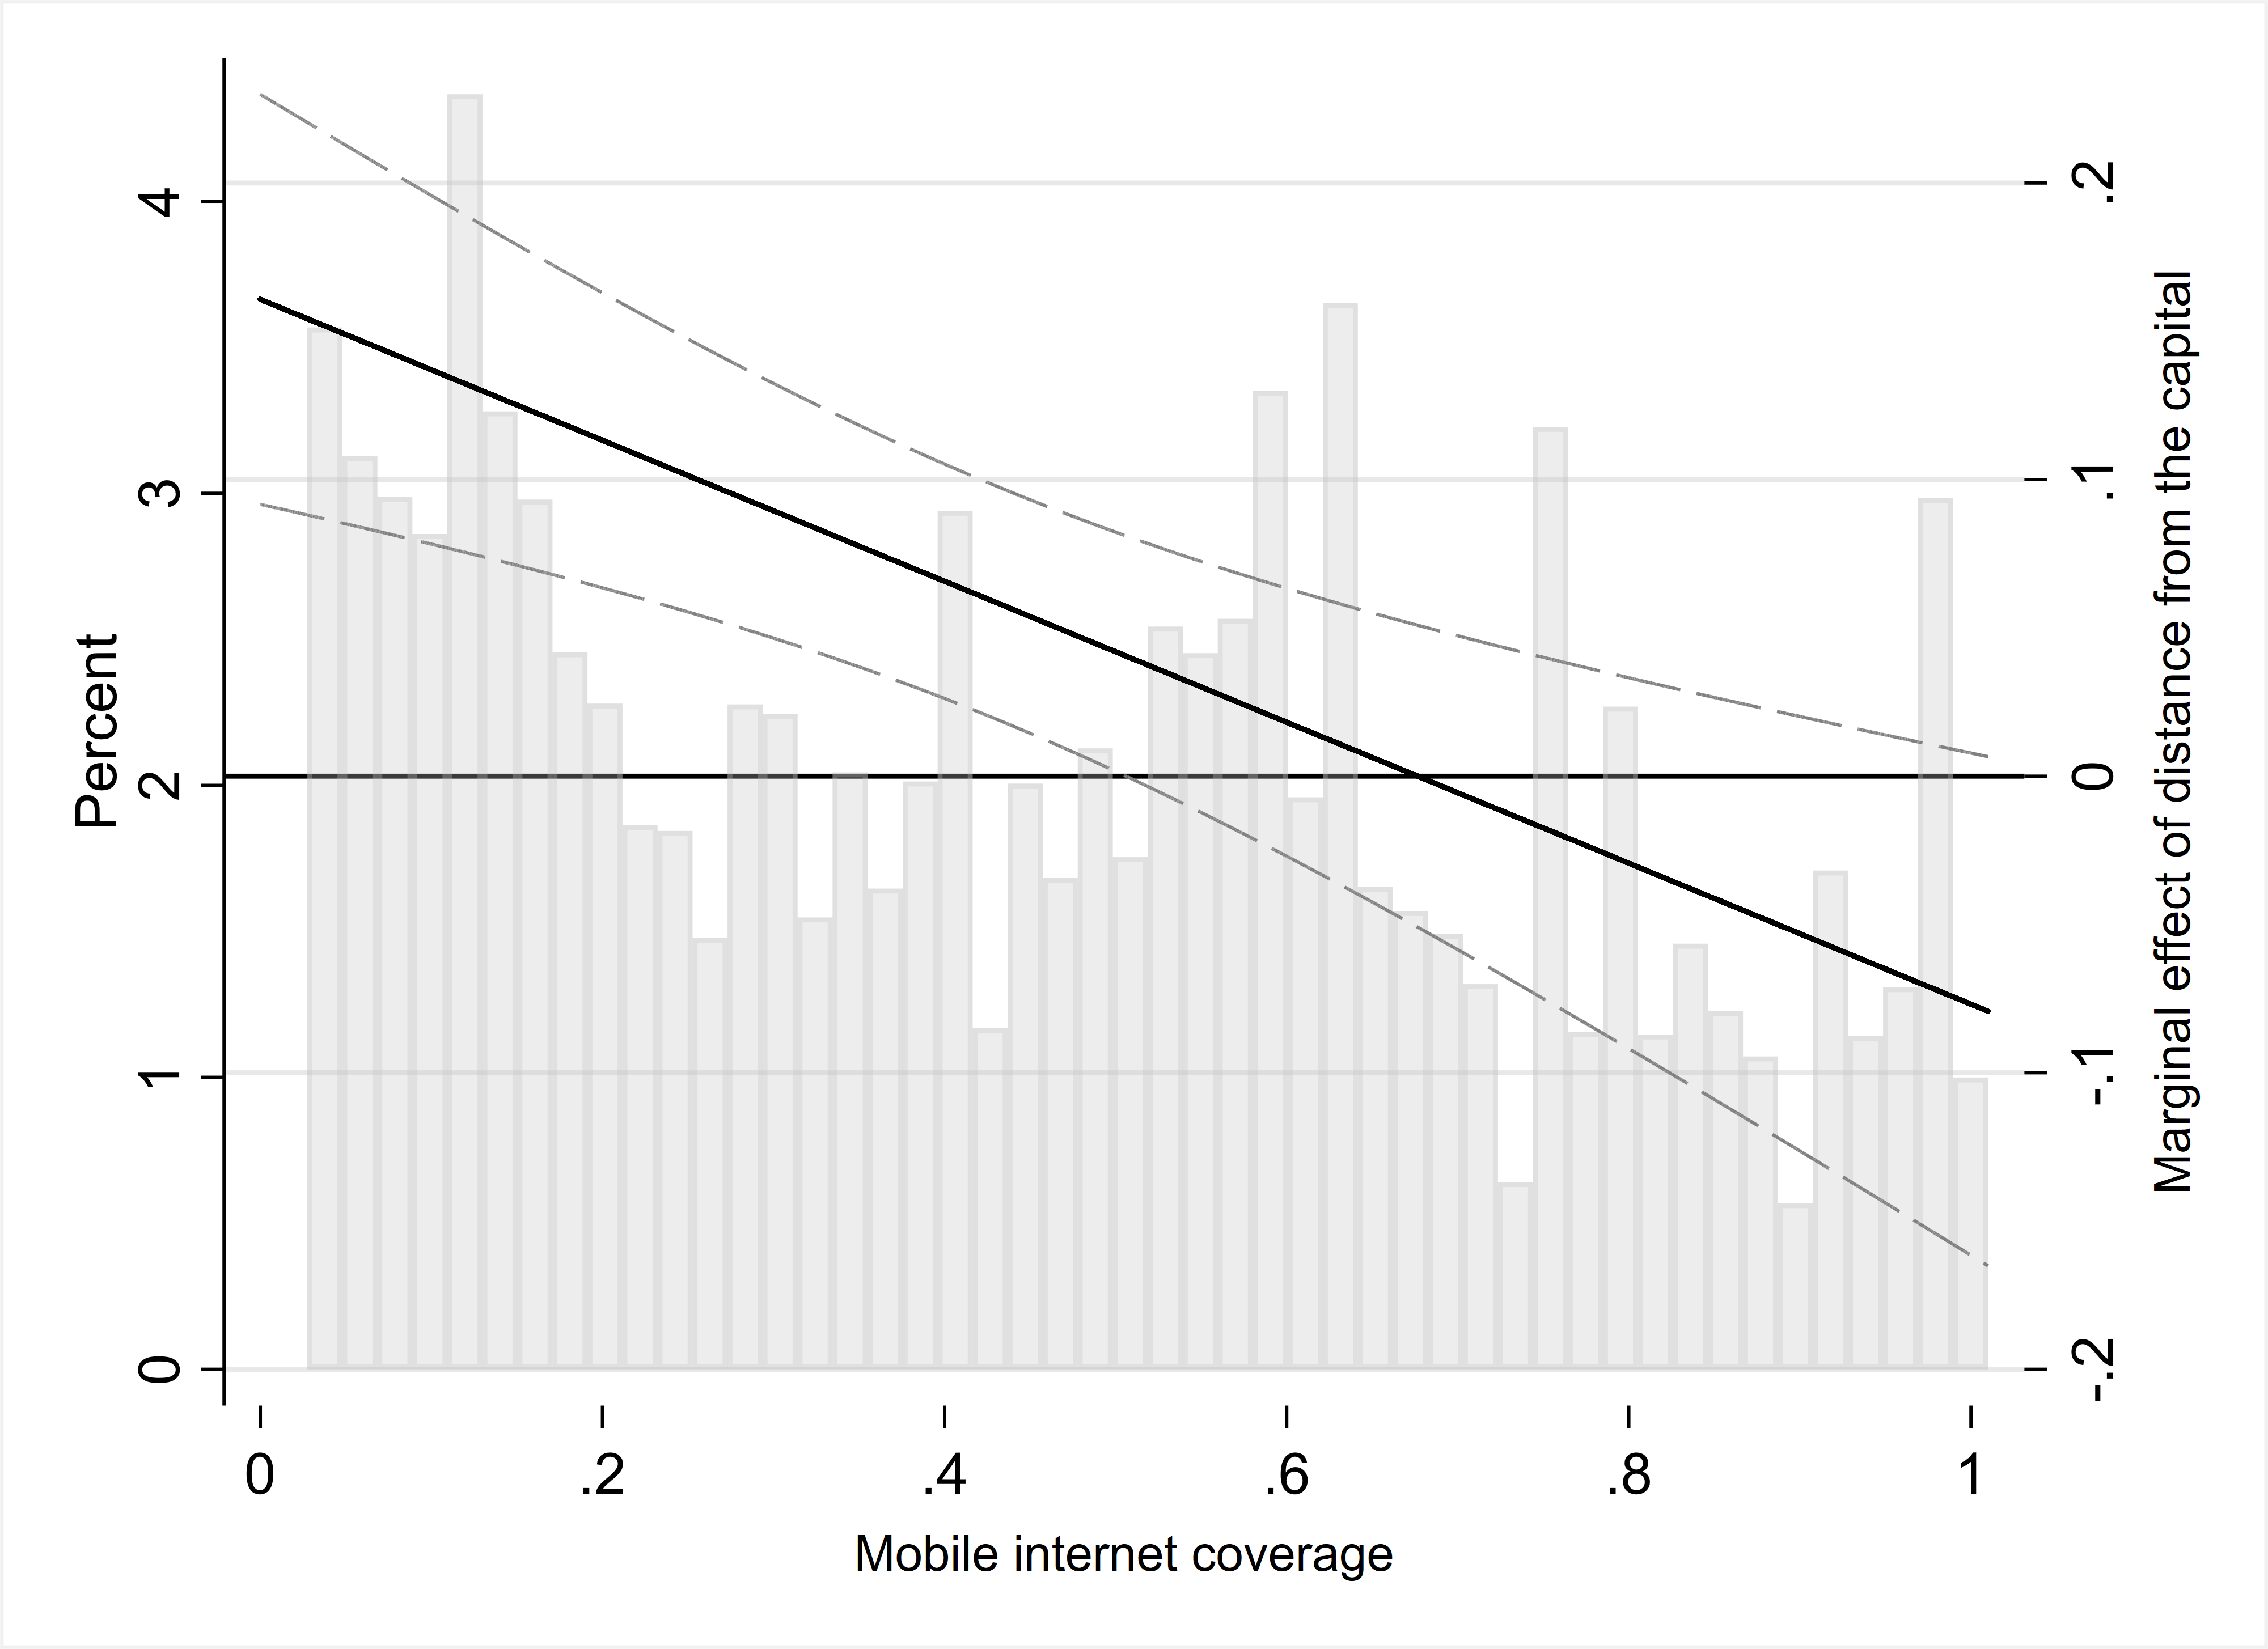
\includegraphics[scale=0.042]{C:/Users/Redha CHABA/Documents/Working paper/trust/script/plots/marginal_effect/vote_oppo.png}
            \caption{Vote against rulling party}
        \end{subfigure}
        \hspace{0.03\textwidth}
        \begin{subfigure}{0.46\textwidth}
            \centering
            \includegraphics[scale=0.042]{C:/Users/Redha CHABA/Documents/Working paper/trust/script/plots/marginal_effect/perf_country.png}
            \caption{Country performance}
        \end{subfigure}
        
    \end{figure}
    
    \end{frame}


    \begin{frame}{Information censorship}
    
    \begin{table}[H]
        \sffamily
        \caption{{Media and institutions freedom}}
        \centering
        %\footnotesize
        \resizebox{10cm}{!}{
        \begin{tabular}{@{\extracolsep{5pt}} l c c c c}
        \\
        \toprule
        \toprule
        & \multicolumn{4}{c}{2SLS: Political trust}\\
        \cmidrule(r){2-5}
        & \multicolumn{4}{c}{{Base sample}}\\
        \cmidrule(r){2-5}
        &\multicolumn{2}{c}{{Media}}&  \multicolumn{2}{c}{{Institutions}}\\
        \cmidrule(r){2-3}
            \cmidrule(r){4-5}
            & \multicolumn{1}{c}{{Free}} & \multicolumn{1}{c}{{Captured}}& \multicolumn{1}{c}{{Free}} & \multicolumn{1}{c}{{Captured}}\\
            \cmidrule(r){2-2}
            \cmidrule(r){3-3}
            \cmidrule(r){4-4}
            \cmidrule(r){5-5}
            & \multicolumn{1}{c}{{(1)}} &  \multicolumn{1}{c}{{(2)}}  & \multicolumn{1}{c}{{(3)}} &  \multicolumn{1}{c}{{(4)}}\\
         \midrule
      
         Distance from the capital&     -4.922   &       1.133*** &       0.078   &       2.151***\\
         \smallskip
         &     (11.77)   &      (0.41)  &      (0.83)   &      (0.77)\\
         Internet coverage        &      -3.475   &       1.220* &       0.112   &       2.964***\\
         \smallskip
         &     (10.01)   &      (0.68)  &      (1.37)   &      (1.06) \\
      Distance from the capital $\times$ Internet coverage&       9.210   &      -2.160* &       0.391   &      -4.202**\\
      \medskip
      &     (21.19)   &      (1.22) &      (1.59)   &      (1.90)\\

    

         \midrule
         \smallskip
        Individual \& regional controls  & Yes & Yes & Yes & Yes\\
        \smallskip
        Country X Round FE       & Yes& Yes & Yes& Yes\\
        \smallskip
        Observations          &       48,174   &       50,061 &       45,238   &       52,997 \\
        \bottomrule
        \multicolumn{5}{p{15cm}}{\footnotesize \emph{Notes}: Robust standard errors clustered at the region x round level are in parentheses. The set of individual controls
        includes values of: normalized distance from the largest non-capital city, age, age squared, sex,
        education, employment status, rural/urban situation, personal economic conditions perception, ethnic discrimination, interest in politics, TV news consumption, newspaper news consumption, radio consumption. The set of regional controls includes values of: nighttime light, population density, region area, president birthplace dummy. *** / ** / * represent significance at the 0.01 / 0.05 / 0.10 levels, respectively.}
        \end{tabular}
        }
        \end{table}
\end{frame}




%\begin{frame}{Internet mitigates spatial disparities}

%    \begin{figure}
%        \includegraphics[scale=0.07]{C:/Users/Redha CHABA/Documents/Working paper/trust/script/plots/marginal_effect/trust_inst_wo_low_cov.png}
%        \caption{Marginal effect of Distance from the capital as a function of Internet coverage}
%    \end{figure}
    
%    \end{frame}

    
%\begin{frame}{Internet mitigates spatial disparities}

%    \begin{figure}
%        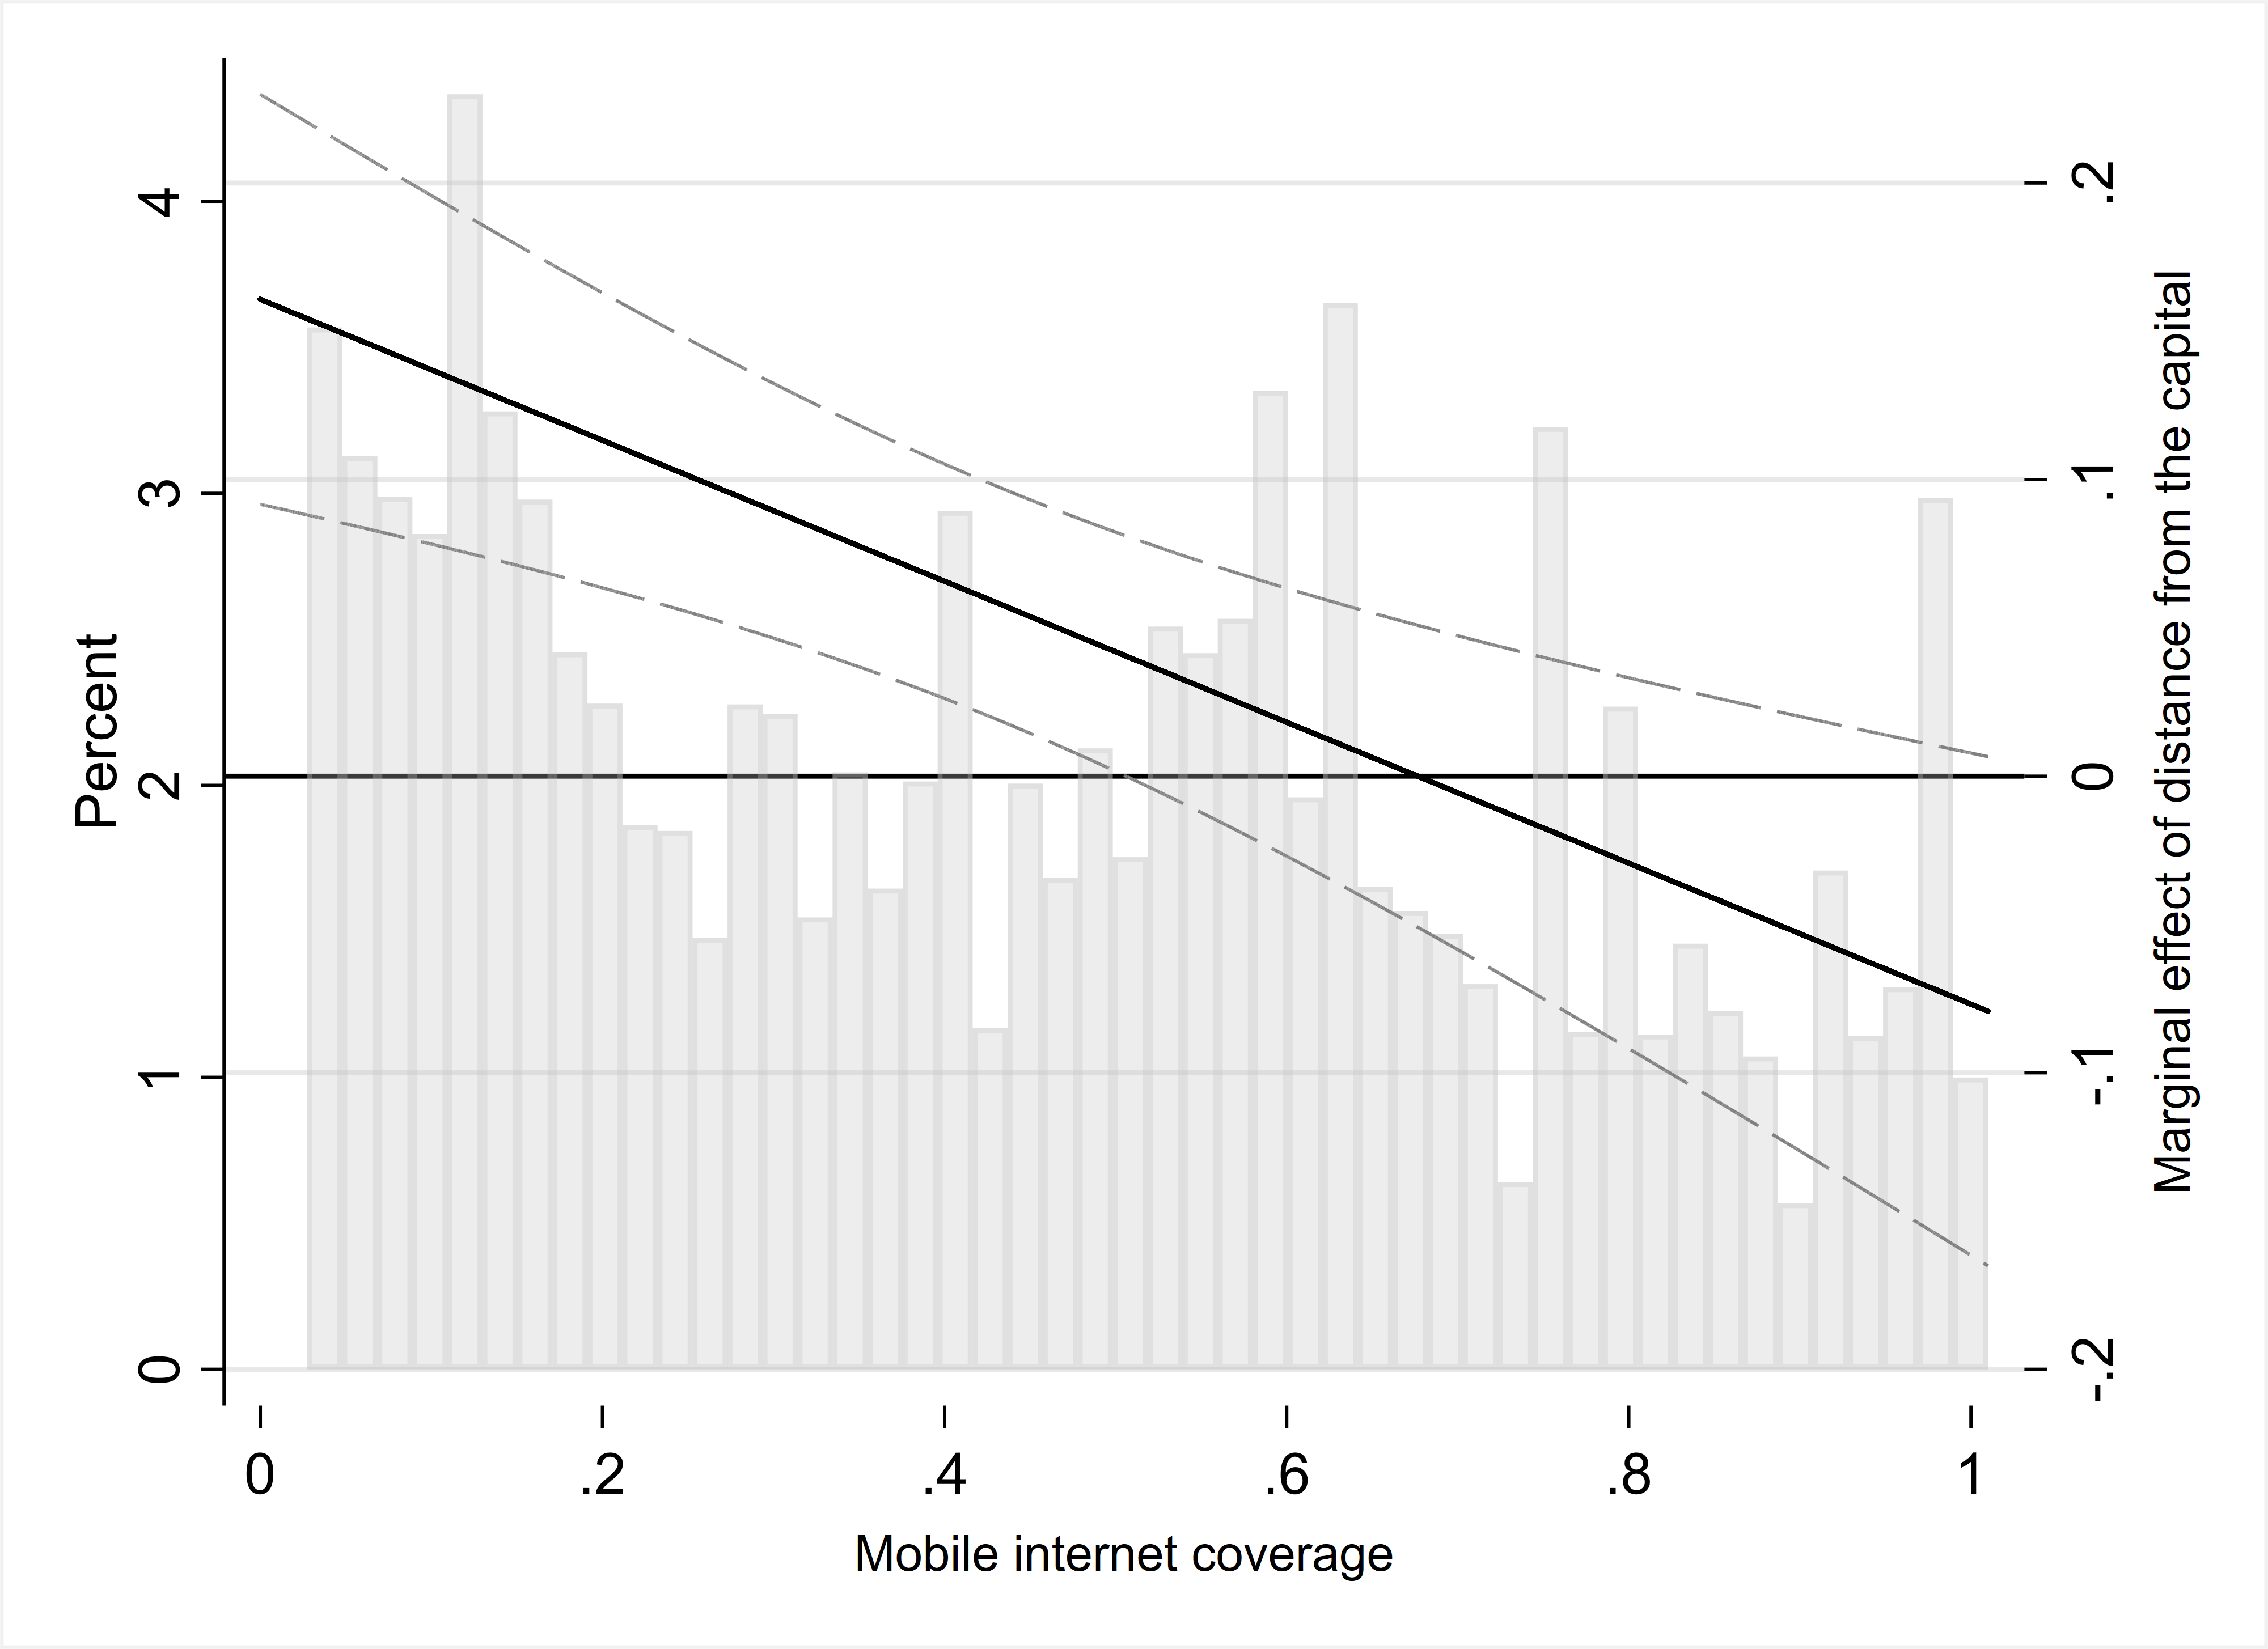
\includegraphics[scale=0.07]{C:/Users/Redha CHABA/Documents/Working paper/trust/script/plots/marginal_effect/vote_oppo.png}
%        \caption{Marginal effect of Distance from the capital as a function of Internet coverage}
%    \end{figure}
    
%    \end{frame}

    
%\begin{frame}{Internet mitigates spatial disparities}

%    \begin{figure}
%        \includegraphics[scale=0.07]{C:/Users/Redha CHABA/Documents/Working paper/trust/script/plots/marginal_effect/vote_oppo_wo_low_cov.png}
%        \caption{Marginal effect of Distance from the capital as a function of Internet coverage}
%    \end{figure}
    
%    \end{frame}

    

    
%\begin{frame}{Internet mitigates spatial disparities}

%    \begin{figure}
%        \includegraphics[scale=0.07]{C:/Users/Redha CHABA/Documents/Working paper/trust/script/plots/marginal_effect/perf_country_wo_low_cov.png}
%        \caption{Marginal effect of Distance from the capital as a function of Internet coverage}
%    \end{figure}
    
%    \end{frame}


\begin{frame}{Conclusion}
    \begin{itemize}\setlength\itemsep{1em}
        \item \textbf{Trust in political institutions} promotes state legitimacy, civic engagement, social cohesion\vfill
        \item \textbf{Nature of trust} is key for expecting favorable outcomes\vfill
        \item High levels of political trust with low information \textbf{can be misleading} and undermine democratic accountability
        and effective governance\vfill
        \item \textbf{Remote areas} are more prone to \textit{uninformed trust} in political institutions due
        to both information scarcity and low expectation-engagement cycle\vfill

    \end{itemize}
\end{frame}

\begin{frame}{Conclusion}

    \begin{itemize}\setlength\itemsep{1em}
        \item \textbf{Mobile internet} potentially breaks information barriers by reducing the
        cost of accessing information about the government\vfill
        \item Replace \textit{uninformed trust} with critical evaluation to restore accountability mechanisms needed for institutional development\vfill
        %\item Stronger effect where the \textbf{government controls} the traditional media and institutions\vfill
    \end{itemize}

\end{frame}

\begin{frame}{IV - Border sample}
    \label{IV-BDD}
    \begin{table}[H]
    \sffamily
    \caption{IV - Border sample : Effect of internet coverage on political trust by distance}
    \centering
    %\footnotesize
    \resizebox{11cm}{!}{
    \begin{tabular}{@{\extracolsep{5pt}} l c c c c c c}
    \\
    \toprule
    \toprule
    & \multicolumn{5}{c}{{Border sample}}\\
    \cmidrule(r){2-6}
    & \multicolumn{1}{c}{{OLS}} & \multicolumn{3}{c}{{First Stage}} & \multicolumn{1}{c}{{2SLS}}\\
        \cmidrule(r){2-2}
        \cmidrule(r){3-5}
        \cmidrule(r){6-6}
        & \multicolumn{1}{c}{{Political trust}} & \multicolumn{1}{c}{{Internet coverage}} & \multicolumn{1}{c}{{}} &  \multicolumn{1}{c}{{Distance $\times$ Internet coverage}} & \multicolumn{1}{c}{{Political trust}}\\
        \cmidrule(r){2-2}
        \cmidrule(r){3-3}
        \cmidrule(r){5-5}    
        \cmidrule(r){6-6}    
        & \multicolumn{1}{c}{{(1)}} & \multicolumn{1}{c}{{(2)}} & \multicolumn{1}{c}{{}} &  \multicolumn{1}{c}{{(3)}} & \multicolumn{1}{c}{{(4)}}\\
        
        \midrule
  
Distance from the capital & 0.640**&&&&  1.214***\\      
\smallskip
&      (0.26)   &&&&     (0.42)   \\
Internet coverage     &      0.620** &&&&       0.809  \\
\smallskip
&  (0.30)   &&&&      (1.02)    \\ 
\smallskip
Distance from the capital $\times$ Internet coverage&      -0.535&&&&       -2.559**\\
\smallskip  &       (0.46)    &&&&      (1.18) \\


Lightning strikes && 0.002 && 0.003***  \\
\smallskip&& (0.00) && (0.00) \\
Distance from the capital city $\times$ Lightning strikes&& 0.000 && -0.003***\\
\medskip&& (0.00) && (0.00)\\

     \midrule
    SW \emph{F} - Lightning strikes &-&-& 12.45 &- &-\\
    \smallskip
    SW \emph{F} - Distance $\times$ Lightning strikes &-&-& 16.25 &-&-\\
    \smallskip
    Individual \& regional controls  & Yes & Yes &&  Yes & Yes\\
    \smallskip
    Country X Round FE       & Yes & Yes&- & Yes & Yes \\
    \smallskip
    Ethnic homeland FE& Yes & Yes&- & Yes & Yes \\
    \smallskip
    Observations       &       4,189    &4,247 && 4,247&      4,189  \\
    Adjusted-R$^2$    &       0.190    &-&-&-&  \\
                          \bottomrule
    \multicolumn{6}{p{21.7cm}}{\footnotesize \emph{Notes}: % Set font size to 8pt with 10pt line spacing
    \emph{Notes}: The border sample includes individuals residing within a 20-kilometer buffer around a country border that overlaps with a historical ethnic homeland, as defined by Murdock (1959). Robust standard errors clustered at the ethnic homeland x region x round level for the border sample are in parentheses. The set of individual controls
    includes values of: normalized distance from the largest non-capital city, age, age squared, sex,
    education, employment status, rural/urban situation, personal economic conditions perception, ethnic discrimination, interest in politics, TV news consumption, newspaper news consumption, radio consumption. The set of regional controls includes values of: nighttime light, population density, region area, president birthplace dummy. *** / ** / * represent significance at the 0.01 / 0.05 / 0.10 levels, respectively.}
\end{tabular}}
    \end{table}

    \hyperlink{IV-Base}{\beamerbutton{IV - Base sample}}

\end{frame}


\begin{frame}{Individual heterogeneity}

    \begin{table}[H]
        \sffamily
        \caption{{Individual heterogeneity}}
        \centering
        %\footnotesize
        \resizebox{10cm}{!}{
        \begin{tabular}{@{\extracolsep{5pt}} l c c c c}
        \\
        \toprule
        \toprule
        & \multicolumn{4}{c}{2SLS: Political trust}\\
        \cmidrule(r){2-5}
        & \multicolumn{4}{c}{{Base sample}}\\
        \cmidrule(r){2-5}
        &\multicolumn{2}{c}{{Education}}&  \multicolumn{2}{c}{{Urban/Rural}}\\
        \cmidrule(r){2-3}
            \cmidrule(r){4-5}
            & \multicolumn{1}{c}{{$<$ Secondary}} & \multicolumn{1}{c}{{$\geq$ Secondary}}& \multicolumn{1}{c}{{Urban}} & \multicolumn{1}{c}{{Rural}}\\
            \cmidrule(r){2-2}
            \cmidrule(r){3-3}
            \cmidrule(r){4-4}
            \cmidrule(r){5-5}
            & \multicolumn{1}{c}{{(1)}} &  \multicolumn{1}{c}{{(2)}}  & \multicolumn{1}{c}{{(3)}} &  \multicolumn{1}{c}{{(4)}}\\
         \midrule
      
         Distance from the capital&       1.208***&       1.394   &       1.133** &       1.961*** \\
         \smallskip
         &      (0.31)   &      (1.17)   &      (0.52)   &      (0.70)  \\
         Internet coverage  &       1.706*  &       1.271   &       0.397   &       3.374***\\
         \smallskip
         &      (0.92)   &      (1.32)   &      (0.63)   &      (1.18)   \\
           Distance from the capital $\times$ Internet coverage&      -1.909** &      -2.422   &      -1.785*  &      -3.447* \\
           \medskip
           &      (0.83)   &      (2.41)   &      (0.98)   &      (1.81)    \\
         \midrule
         \smallskip
        Individual \& regional controls  & Yes & Yes & Yes & Yes\\
        \smallskip
        Country X Round FE       & Yes& Yes & Yes& Yes\\
        \smallskip
        Observations         &       36,389   &       62,039   &       37,348   &       60,887\\
        \bottomrule
        \multicolumn{5}{p{15cm}}{\footnotesize \emph{Notes}: Robust standard errors clustered at the region x round level are in parentheses. The set of individual controls
        includes values of: normalized distance from the largest non-capital city, age, age squared, sex,
        education, employment status, rural/urban situation, personal economic conditions perception, ethnic discrimination, interest in politics, TV news consumption, newspaper news consumption, radio consumption. The set of regional controls includes values of: nighttime light, population density, region area, president birthplace dummy. Education, rural/urban, and age controls are omitted from columns (1-2), (3-4), and (5-8), respectively.*** / ** / * represent significance at the 0.01 / 0.05 / 0.10 levels, respectively.}
        \end{tabular}
        }
        \end{table}
\end{frame}




\begin{frame}{IV - Internet news}
    \begin{table}[H]
    \sffamily
    \caption{IV - Base sample : Effect of internet news on political trust by distance}
    \centering
    %\footnotesize
    \resizebox{11cm}{!}{
    \begin{tabular}{@{\extracolsep{5pt}} l c c c c c c}
    \\
    \toprule
    \toprule
    & \multicolumn{5}{c}{{Border sample}}\\
    \cmidrule(r){2-6}
    & \multicolumn{1}{c}{{OLS}} & \multicolumn{3}{c}{{First Stage}} & \multicolumn{1}{c}{{2SLS}}\\
        \cmidrule(r){2-2}
        \cmidrule(r){3-5}
        \cmidrule(r){6-6}
        & \multicolumn{1}{c}{{Political trust}} & \multicolumn{1}{c}{{Internet news}} & \multicolumn{1}{c}{{}} &  \multicolumn{1}{c}{{Distance $\times$ Internet news}} & \multicolumn{1}{c}{{Political trust}}\\
        \cmidrule(r){2-2}
        \cmidrule(r){3-3}
        \cmidrule(r){5-5}    
        \cmidrule(r){6-6}    
        & \multicolumn{1}{c}{{(1)}} & \multicolumn{1}{c}{{(2)}} & \multicolumn{1}{c}{{}} &  \multicolumn{1}{c}{{(3)}} & \multicolumn{1}{c}{{(4)}}\\
        
        \midrule
  
Distance from the capital & 0.301***&&&&       0.768***\\      
\smallskip
&      (0.03)   &&&&      (0.12)   \\
Internet news     &      -0.010*  &&&&      -0.308  \\
\smallskip
&    (0.01)   & &&&     (0.23)    \\ 
\smallskip
Distance from the capital $\times$ Internet news&      -0.045***&&&&      -0.800***\\
\smallskip  &       (0.01)    &&&&      (0.17) \\


Internet coverage &&  0.253*** && -0.129***  \\
\smallskip&& (0.057) && (0.037) \\
Distance from the capital city $\times$ Internet coverage&& -0.077 && 0.622***\\
\medskip&& (0.09) && (0.07)\\

     \midrule
    SW \emph{F} - Internet coverage &-&-& 28.25 &- &-\\
    \smallskip
    SW \emph{F} - Distance $\times$ Internet coverage &-&-& 81.36 &-&-\\
    \smallskip
    Individual \& regional controls  & Yes & Yes &&  Yes & Yes\\
    \smallskip
    Country X Round FE       & Yes & Yes&- & Yes & Yes \\
    \smallskip
    Ethnic homeland FE& Yes & Yes&- & Yes & Yes \\
    \smallskip
    Observations       &       97,686    &98,849&& 98,849&      97,686  \\
    Adjusted-R$^2$    &       0.198     &-&-&-&  \\
                          \bottomrule
    \multicolumn{6}{p{21.7cm}}{\footnotesize \emph{Notes}: % Set font size to 8pt with 10pt line spacing
    \emph{Notes}: Robust standard errors clustered at the x region x round level are in parentheses. The set of individual controls
    includes values of: normalized distance from the largest non-capital city, age, age squared, sex,
    education, employment status, rural/urban situation, personal economic conditions perception, ethnic discrimination, interest in politics, TV news consumption, newspaper news consumption, radio consumption. The set of regional controls includes values of: nighttime light, population density, region area, president birthplace dummy. *** / ** / * represent significance at the 0.01 / 0.05 / 0.10 levels, respectively.}
\end{tabular}}
    \end{table}
\end{frame}



\begin{frame}{IV - Social media news}
    \begin{table}[H]
    \sffamily
    \caption{IV - Base sample : Effect of social media news on political trust by distance}
    \centering
    %\footnotesize
    \resizebox{11cm}{!}{
    \begin{tabular}{@{\extracolsep{5pt}} l c c c c c c}
    \\
    \toprule
    \toprule
    & \multicolumn{5}{c}{{Border sample}}\\
    \cmidrule(r){2-6}
    & \multicolumn{1}{c}{{OLS}} & \multicolumn{3}{c}{{First Stage}} & \multicolumn{1}{c}{{2SLS}}\\
        \cmidrule(r){2-2}
        \cmidrule(r){3-5}
        \cmidrule(r){6-6}
        & \multicolumn{1}{c}{{Political trust}} & \multicolumn{1}{c}{{Social medias news}} & \multicolumn{1}{c}{{}} &  \multicolumn{1}{c}{{Distance $\times$ Social medias news}} & \multicolumn{1}{c}{{Political trust}}\\
        \cmidrule(r){2-2}
        \cmidrule(r){3-3}
        \cmidrule(r){5-5}    
        \cmidrule(r){6-6}    
        & \multicolumn{1}{c}{{(1)}} & \multicolumn{1}{c}{{(2)}} & \multicolumn{1}{c}{{}} &  \multicolumn{1}{c}{{(3)}} & \multicolumn{1}{c}{{(4)}}\\
        
        \midrule
  
Distance from the capital & 0.340***&&&&       0.656***\\      
\smallskip
&       (0.04)   &&&&      (0.13)   \\
Social medias news     &       -0.013** &&&&      -0.623  \\
\smallskip
&     (0.01)   &&&&      (0.38)    \\ 
\smallskip
Distance from the capital $\times$ Social medias news&      -0.045***&&&&       -0.500***\\
\smallskip  &       (0.01)    &&&&      (0.15)   \\


Internet coverage && 0.212*** && -0.249***  \\
\smallskip&& (0.07) && (0.05) \\
Distance from the capital city $\times$ Internet coverage&& -0.120 && 0.949***\\
\medskip&& (0.11) && (0.09)\\

     \midrule
    SW \emph{F} - Internet coverage &-&-&  10.39 &- &-\\
    \smallskip
    SW \emph{F} - Distance $\times$ Internet coverage &-&-& 63.93 &-&-\\
    \smallskip
    Individual \& regional controls  & Yes & Yes &&  Yes & Yes\\
    \smallskip
    Country X Round FE       & Yes & Yes&- & Yes & Yes \\
    \smallskip
    Ethnic homeland FE& Yes & Yes&- & Yes & Yes \\
    \smallskip
    Observations       &        70,234     &71,103&& 71,103&       70,234   \\
    Adjusted-R$^2$    &        0.207     &-&-&-&  \\
                          \bottomrule
    \multicolumn{6}{p{21.7cm}}{\footnotesize \emph{Notes}: % Set font size to 8pt with 10pt line spacing
    \emph{Notes}: Robust standard errors clustered at the x region x round level are in parentheses. The set of individual controls
    includes values of: normalized distance from the largest non-capital city, age, age squared, sex,
    education, employment status, rural/urban situation, personal economic conditions perception, ethnic discrimination, interest in politics, TV news consumption, newspaper news consumption, radio consumption. The set of regional controls includes values of: nighttime light, population density, region area, president birthplace dummy. *** / ** / * represent significance at the 0.01 / 0.05 / 0.10 levels, respectively.}
\end{tabular}}
    \end{table}

\end{frame}



\begin{frame}{Country sample and capital cities}
\label{sample_map}
    \begin{figure}
        \centering
        \caption{Country Sample and Capital Cities}
        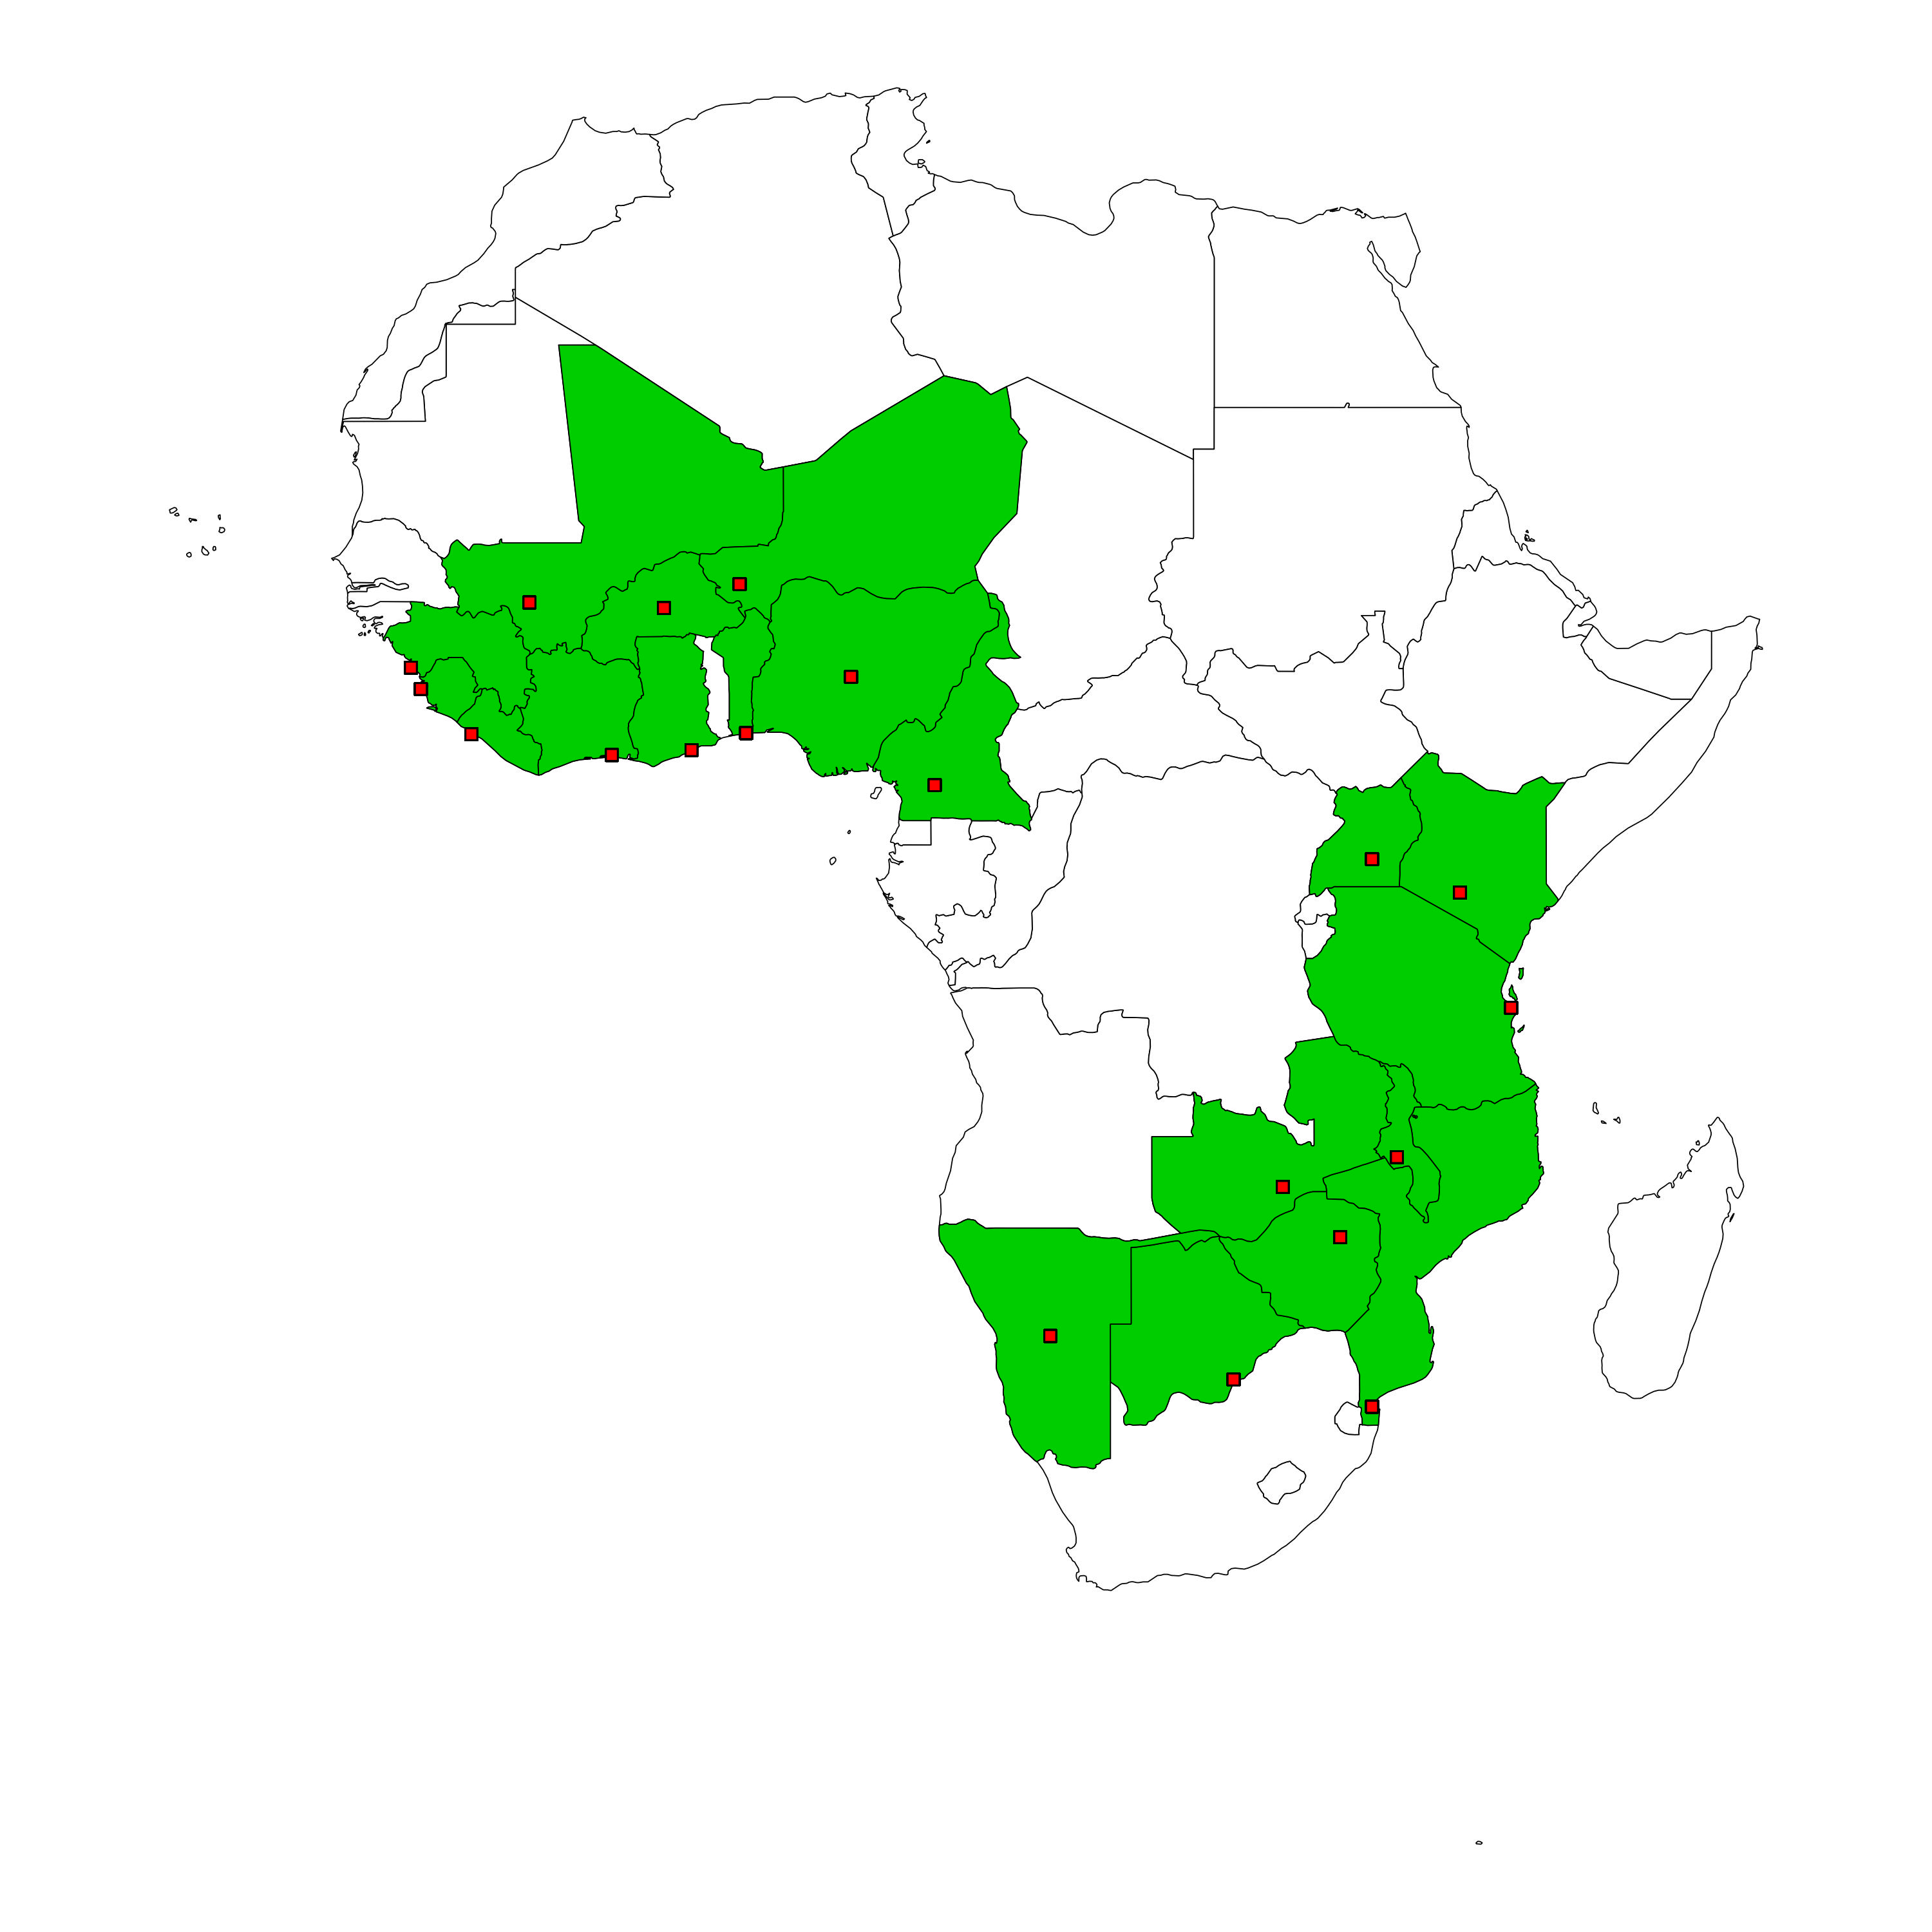
\includegraphics[scale=0.075]{obs_map.jpg}
    \end{figure}

    \begin{tikzpicture}[remember picture, overlay]
        \node[anchor=south west] at (current page.south west) [xshift=1cm, yshift=0.5cm] {%
            \hyperlink{context}{\beamerbutton{Back}}};
    \end{tikzpicture}
    
\end{frame}

\end{document}